\documentclass[11pt,twoside]{article}
\usepackage{latex-macros/course}

%\renewcommand{\coursecopyrightyear}{2002}

\begin{document}
\lecturenotes{11-12}{Random Variables and Expectation}

\section{Random Variables}
 
When we perform an experiment, we expect the results to be observable
---did the player hit a home run or not?---or measurable---how far did
the ball travel? how fast was the pitch?  To describe the behavior of such
probabilistic experiments with measurable outcomes, we use \emph{random
  variables}.

For example, tossing three independent, unbiased coins allows
definition of two random variables: $C$ is defined to be the number of
heads and $M$ is defined to be 1 iff all three coins match and 0
otherwise.  Any outcome of the coin flips uniquely determines $C$ and
$M$.  $C$ can take the values 0,1,2, and 3, and $M$ the values $0$ an
$1$.

We use the notation $[C = 2]$ for the event that there are two heads.
Similarly, $[C \geq 2]$ is the event that there are at least two heads,
and $[C \in \set{1, 3}]$ is the event that there are an odd number of
heads.

Now consider the event that the product of $C$ and $M$ is positive; we
write this one as $[C \cdot M >0]$.  Since neither $C$ nor $M$ take
negative values, $C\cdot M>$ iff both $C>0$ and $M>0$---in other words,
there is a head, and all three dice match.  So saying $C \cdot M >0$ is
just an obscure way of saying that all three coin flips come up heads.
That is, the event $[C \cdot M >0]$ consists of the single outcome
\texttt{HHH}.

When the meaning is clear, we often omit the square brackets denoting
events.  For example, we say ``the event $C=0$'' instead of ``the event
$[C=0]$,'' or $\pr{C=0}$ instead of $\pr{[C=0]}$.

Saying that each outcome uniquely determines $C$ and $M$ means that we can
think of $C$ and $M$ as functions from outcomes to their values.  The
natural sample space $\sspace$ for this experiment consists of eight
outcomes: $\mathtt{HHH}$, $\mathtt{HHT}$, $\mathtt{HTH}$, \etc.  For
example, $C(\mathtt{HHH}) = 3$, $C(\mathtt{HTH}) = 2$, $C(\mathtt{TTT}) =
0$.  Similarly, $M(\mathtt{HHH}) = 1$, $M(\mathtt{HTH}) = 0$,
$M(\mathtt{TTT}) = 1$.

We can formalize the idea of a random variable in general as follows.
\begin{definition}
A \emph{random variable} over a given sample space is a function that maps
every outcome to a real number.
\end{definition}

Notice that calling a random variable a ``variable'' a misnomer: it is
actually a function.

We will use the random variables $C$ and $M$ as continuing examples.  Keep
in mind that $C$ \textbf{\emph{c}}ounts heads and $M$ indicates that all
coins \textbf{\emph{m}}atch.

\subsection{Indicator Random Variables}

\emph{Indicator} random variables describe experiments to detect whether
or not something happened.  The random variable $M$ is an example of an
indicator variable, indicating whether or not all three coins match.

\begin{definition}
An \emph{indicator random variable} is a random variable that maps
every outcome to either 0 or 1.
\end{definition}

Indicator random variables are also called \emph{Bernoulli} or
\emph{characteristic} random variables.  Typically, indicator random
variables identify all outcomes that share some property
(``characteristic''): outcomes with the property are mapped to 1, and
outcomes without the property are mapped to 0.

\subsection{Events Defined by a Random Variable}

There is a natural relationship between random variables and events.
Recall that an event is just a subset of the outcomes in the sample
space of an experiment.

The relationship is simplest for an indicator random variable.  An
indicator random variable partitions the sample space into two blocks:
outcomes mapped to 1 and outcomes mapped to~0.  These two sets of outcomes
are events.  For example, the random variable $M$ partitions the sample
space as follows:
\[
\underbrace{\mathtt{HHH} \quad \mathtt{TTT}}_{\mbox{mapped to 1}} \quad
\underbrace{\mathtt{HHT} \quad \mathtt{HTH} \quad \mathtt{HTT} \quad
        \mathtt{THH} \quad \mathtt{THT} \quad \mathtt{TTH}}_{\mbox{mapped to 0}}
\]
Thus, the random variable $M$ defines two events, the event $[M = 1]$ that
all coins match and the event $[M = 0]$ that not all coins match.

The random variable $C$ partitions the sample space into four blocks:
\[
\underbrace{\mathtt{TTT}}_{\mbox{mapped to 0}} 
\underbrace{\mathtt{TTH} \quad \mathtt{THT} \quad \mathtt{HTT}}_{\mbox{mapped to 1}} \quad
\underbrace{\mathtt{THH} \quad \mathtt{HTH} \quad \mathtt{HHT}}_{\mbox{mapped to 2}} \quad
\underbrace{\mathtt{HHH}}_{\mbox{mapped to 3}} 
\]
Thus, the random variable $C$ defines the four events $[C=i]$ for $i \in
\set{0, 1, 2, 3}$.  These are the events that no coin is heads, that one
coin is heads, that two coins are heads, and finally that three coins are
heads.

A general random variable may partition the sample space into many blocks.
A block contains all outcomes mapped to the same value by the random
variable.

\iffalse
In general, suppose $P(r_1,\dots,r_n)$ is a proposition about real numbers
$r_1,\dots,r_n$, and $R_1,\dots,R_n$ are random variables.  Then we use
the notation $[P(R_1,\dots,R_n)]$ to denote the event that the values of
$R_1,\dots,R_n$ satisfy $P$.  That is,
\[
[P(R_1,\dots,R_n)] \eqdef \set{ w \in \sspace \suchthat P(R_1(w),\dots,R_n(w))}.
\]
\fi

\subsection{Probability of Events Defined by a Random Variable}

Recall that the probability of an event is the sum of the probabilities of
the outcomes it contains.  From this rule, we can compute the probability
of various events associated with a random variable.  For example, if $R :
\sspace \to \reals$ is a random variable and $x$ is a real number, then
\begin{equation*}
\pr{R = x}  =  \sum_{w \in [R = x]} \pr{w}.
\end{equation*}
For example, we can compute $\pr{C = 2}$ as follows:
\begin{align*}
\pr{C = 2} = & \sum_{w \in [C = 2]} \pr{w} & \text{(def of $\pr{}$)}\\
           = & \pr{\mathtt{THH}} + \pr{\mathtt{HTH}}
               + \pr{\mathtt{HHT}} \text{(the 3 outcomes in $[C=2]$)}\\
           = & \frac{1}{8} + \frac{1}{8} + \frac{1}{8} = \frac{3}{8}.
\end{align*}
Note that each outcome has probability $1/8$, since the three coins are
fair and independent.

Similarly, we can compute $\pr{M = 1}$ and $\pr{C \geq 2}$
\begin{eqnarray*}
\pr{M = 1}      & = & \sum_{w \in [M = 1]} \pr{w} \\
                & = & \pr{\mathtt{HHH}} + \pr{\mathtt{TTT}}\\
                & = & \frac{1}{8} + \frac{1}{8} = \frac{1}{4}.
\\
\pr{C \geq 2}   & = &   \sum_{w \in [C \geq 2]} \pr{w} \\
                & = &   \pr{\mathtt{THH}} + \pr{\mathtt{HTH}} + \pr{\mathtt{HHT}} + \pr{\mathtt{HHH}} \\
             & = &   \frac{1}{8}+\frac{1}{8}+\frac{1}{8}+\frac{1}{8} = \frac{1}{2}.
\end{eqnarray*}
The justification for each step is the same as before.

It's common in such calculations to group outcomes by their value.
For instance, we could also have calculated:
\begin{eqnarray*}
\pr{C \geq 2}   & = &   \pr{C = 2} + \pr{C = 3} \\
                & = &   \pr{\mathtt{THH}, \mathtt{HTH}, \mathtt{HHT}} + \pr{\mathtt{HHH}} \\
                & = &   \frac{3}{8}+\frac{1}{8} = \frac{1}{2}
\end{eqnarray*}

\iffalse
If the range of $R$ is $\set{a_0,a_1,\dots} \subset \reals$, an expression
of the form $\pr{R \geq x}$ can also be evaluated with the summation
$\sum_{a_i \geq x} \pr{R = a_i}$.  That is, instead of summing over outcomes
mapped to at least $x$ as above, we can sum probabilities over all values
of the random variable that are greater than or equal to $x$.  The result
is the same, since both summations cover the same outcomes.
\fi

Similarly, we find the probability of the event that $C \in \set{ 1, 3}$.
\iffalse
\begin{eqnarray*}
\pr{C \in \{1, 3 \}}
        & = &   \sum_{w \in [C \in \set{1, 3}]} \pr{w} \\
        & = &   \pr{\mathtt{TTH}}+\pr{\mathtt{THT}}+\pr{\mathtt{HTT}} + \pr{\mathtt{HHH}} \\
        & = &   \frac{1}{8} + \frac{1}{8} + \frac{1}{8} + \frac{1}{8} = \frac{1}{2}.
\end{eqnarray*}

As in the preceding example, this probability could be evaluated by
summing probabilities over values of $C$ instead of by summing over
outcomes:
\fi
\begin{eqnarray*}
\pr{C \in \{1, 3 \}} & = &   \pr{C = 1} + \pr{C = 3} \\
                     & = &   \pr{\mathtt{TTH}, \mathtt{THT}, \mathtt{HTT}}
                              + \pr{\mathtt{HHH}} \\
        & = &   \frac{3}{8}+\frac{1}{8} = \frac{1}{2}.
\end{eqnarray*}

In general, for a set $A = \set{a_0,a_1,\dots}$ of real numbers, $\pr{R
\in A}$ can also be evaluated by summing over the values in $A$.  That is,
\[
\pr{R \in A} = \sum_{a \in A} \pr{R = a}.
\]

\subsection{Conditional Probability}

Mixing conditional probabilities and events involving random variables
creates no new difficulties.  For example, $\prcond{C \geq 2}{M = 0}$
is the probability that at least two coins are heads ($C \geq 2$),
given that all three coins are not the same ($M = 0$).  We can compute
this probability using the familiar Product Rule:

\begin{eqnarray*}
\prcond{C \geq 2}{M = 0}
        & = &   \frac{\pr{C \geq 2 \land M = 0}}{\pr{M = 0}} \\
        & = &   \frac{\pr{\set{\mathtt{THH}, \mathtt{HTH}, \mathtt{HHT}}}}
                     {\pr{\set{\mathtt{THH}, \mathtt{HTH}, \mathtt{HHT},
                             \mathtt{HTT}, \mathtt{THT}, \mathtt{TTH}}}} \\
        & = &   \frac{3/8}{6/8} =  \frac{1}{2}.
\end{eqnarray*}

\subsection{Independence}

\iffalse
The notion of independence does not carry over to random variables so
easily.  In analogy to event independence, we will first define
independence for a pair of random variables and then define mutual
independence for two or more random variables.
\fi

\subsubsection{Independence for Two Random Variables}

\begin{definition}\label{ind1}
Two random variables $R_1$ and $R_2$ are \emph{independent}\footnote{This
definition works for sample spaces $\sspace = \set{w_0,w_1,\dots}$ of the
kind we consider in 6.042.  For more general sample spaces, the definition
is that
\[
\prcond{y_1 \le R_1  \le x_1}{y_2 \le R_2 \le x_2} =
                         \pr{y_1 \le R_1 \le x_1}
\]
for all $y_1,x_1,y_2, x_2 \in \reals$ and $\pr{y_2 \le R_2 \le x_2} \neq 0$.}
if for all $x_1, x_2 \in \reals$ such that $\pr{R_2 = x_2} \neq 0$,
we have:
\[
\prcond{R_1 = x_1}{R_2 = x_2} = \pr{R_1 = x_1}
\]
\end{definition}

As with independence of events, we can also formulate independence of two
random variables in terms of the conjunction of events:
\begin{definition}\label{ind2}
Two random variables $R_1$ and $R_2$ are \emph{independent} if for all
$x_1, x_2 \in \reals$ , we have:
\[
\pr{R_1 = x_1 \land R_2 = x_2} = \pr{R_1 = x_1} \cdot \pr{R_2 = x_2}.
\]
\end{definition}

Definition~\ref{ind1} says that the probability that $R_1$ has a
particular value is unaffected by the value of $R_2$, reflecting the
intuition behind independence.  Definition~\ref{ind2} has the slight
technical advantage that it applies even if $\pr{R_2 = x_2} = 0$.
Otherwise, the two definitions are equivalent, and we will use them
interchangably.

\subsubsection{Proving that Two Random Variables are Not Independent}

Are $C$ and $M$ independent?  Intuitively, no: the number of heads $C$
not only affects, but completely determines whether all three coins match,
that is, whether $M = 1$.  To verify this, let's use the first
definition~\ref{ind1} of independence.  We must find some $x_1, x_2 \in
\reals$ such that the condition in the first definition is false.  For
example, the condition does not hold for $x_1 = 2$ and $x_2 = 1$:
\begin{eqnarray*}
\pr{C = 2 \land M = 1} = 0
        & \mbox{ but } &
\pr{C = 2} \cdot \pr{M = 1} = \frac{3}{8} \cdot \frac{1}{4} \neq 0
\end{eqnarray*}

The first probability is zero because we never have exactly two heads ($C
= 2$) when all three coins match ($M = 1$).  The other two probabilities
were computed earlier.

\subsubsection{A Dice Example}

Suppose that we roll two fair, independent dice.  We can regard the
numbers that turn up as random variables $D_1$ and $D_2$.  For
example, if the outcome is $w = (3, 5)$, then $D_1(w) = 3$ and $D_2(w)
= 5$.

Let $T = D_1 + D_2$.  Then $T$ is also a random variable, since it is
a function mapping each outcome to a real number, namely the sum of
the numbers shown on the two dice.  For outcome $w = (3, 5)$, we have
$T(w) = 3 + 5 = 8$.

Define $S$ as follows:
\[
S \eqdef \left\{
\begin{array}{cl}
1 & \mbox{if $T = 7$}, \\
0 & \mbox{if $T \neq 7$}.
\end{array}
\right.
\]
That is, $S = 1$ if the sum of the dice is 7, and $S = 0$ if the sum
of the dice is not 7.  For example, for outcome $w = (3, 5)$, we have
$S(w) = 0$, since the sum of the dice is 8.  Since $S$ is a function
mapping each outcome to a real number, $S$ is also a random variable.
In particular, $S$ is an indicator random variable, since every
outcome is mapped to 0 or 1.

The definitions of random variables $T$ and $S$ illustrate a general
rule: \emph{any function of random variables is also random variable}.

Are $D_1$ and $T$ independent?  That is, is the sum $T$ of the two dice
independent of the outcome $D_1$ of the first die?  Intuitively, the
answer appears to be no.  To prove this, let's use the
Definition~\ref{ind2} of independence.  We must find $x_1, x_2 \in \reals$
such that $\pr{x_2} \neq 0$ and the condition in the second definition
does not hold.

For example, we can choose $x_1 = 2$ and $x_2 = 3$:
\[
\prcond{T = 2}{D_1 = 3} = 0 \neq \frac{1}{36} = \pr{T = 2}.
\]
The first probability is zero, since if we roll a three on the first die
($D_1 = 3$), then there is no way that the sum of both dice is two ($T =
2$).  On the other hand, if we throw both dice, the probability that the
sum is two is $1/36$, since we could roll two ones.

Are $S$ and $D_1$ independent?  That is, is the probability of the event
$S$ that the sum of both dice is seven independent of the outcome $D_1$
of the first die?  Once again, intuition suggests that the answer is
``no''.  Surprisingly, however, these two random variables \emph{are}
actually independent!

Proving that two random variables are independent requires some work.
Let's use Definition~\ref{ind1} of independence based on conditional
probability.  We must show that for all $x_1, x_2$ in $\reals$ such that
$\pr{D_1 = x_2} \neq 0$:
\[
\prcond{S = x_1}{D_1 = x_2} = \pr{S = x_1}.
\]

First, notice that we only have to show the equation for values of $x_2$
such that $\pr{D_1 = x_2} \neq 0$.  This means we only have to consider
$x_2$ equal to 1, 2, 3, 4, 5, or 6.  If $x_1$ is neither 0 nor 1, then the
condition holds trivially because both sides are zero.  So it remains to
check the equation for the cases where $x_1 \in \set{0, 1}$ and $x_2 \in
\set{ 1,2,3,4,5,6}$, that is, a total of $2 \cdot 6 = 12$ cases.

Two observations make this easier.  First, there are $6 \cdot 6 = 36$
outcomes in the sample space for this experiment.  The outcomes are
equiprobable, so each outcome has probability $1/36$.  The two dice
sum to seven in six outcomes: $1+6$, $2+5$, $3+4$, $4+3$, $5+2$ and
$6+1$.  Therefore, the probability $\pr{S = 1}$ of rolling a seven is
$6/36 = 1/6$.

Second, after we know the result of the first die, there is always exactly
one value for the second die that makes the sum seven.  For example, if
the first die is 2, then the sum is seven only if the second die is a 5.
Therefore, $\prcond{S = 1}{D_1 = x_2} = 1/6$ for $x_2 = 1, 2, 3, 4, 5,$ or
$6$.

These two observations establish the independence condition in six
cases:
\begin{eqnarray*}
\prcond{S = 1}{D_1 = 1} = & \cfrac{1}{6} & = \pr{S = 1} \\
\prcond{S = 1}{D_1 = 2} = & \cfrac{1}{6} & = \pr{S = 1} \\
                    &    \vdots   &  \\
\prcond{S = 1}{D_1 = 6} = & \cfrac{1}{6} & = \pr{S = 1}
\end{eqnarray*}
The remaining cases are complementary to the the first six.  For
example, we know that $\pr{S = 0} = 5/6$, since the
complementary event $S = 1$ has probability $1/6$.
\begin{eqnarray*}
\prcond{S = 0}{D_1 = 1} = & \cfrac{5}{6} & = \pr{S = 0} \\
\prcond{S = 0}{D_1 = 2} = & \cfrac{5}{6} & = \pr{S = 0} \\
                    &    \vdots   &  \\
\prcond{S = 0}{D_1 = 6} = & \cfrac{5}{6} & = \pr{S = 0}
\end{eqnarray*}

We have established that the independence condition holds for all
necessary $x_1, x_2 \in \reals$.  This proves that $S$ and $D_1$ are
independent after all!

\subsubsection{Mutual Independence}

The definition of mutual independence for random variables is similar
to the definition for events.

\begin{definition}
Random variables $R_1, R_2, \dots$ are \emph{mutually independent} iff
\[
\pr{\lgintersect_{i} [R_i = x_i]} = \prod_{i} \pr{R_i = x_i},
\]
for all $x_1, x_2, \dots \in \reals$.
\end{definition}

For example, consider the experiment of throwing three independent, fair
dice.  Random variable $R_1$ is the value of the first die.  Random
variable $R_2$ is the sum of the first two dice, mod 6.  Random variable
$R_3$ is the sum of all three values, mod 6.  These three random variables
are mutually independent.  Can you prove it?

\section{Probability Density Functions}

A random variable is a function from the sample space of an experiment to
the real numbers.  As a result, every random variable is bound up in some
particular experiment.  Often, however, we want to describe a random
variable independent of any experiment.  This consideration motivates the
notion of a \emph{probability density function}.

%%\subsection{Definitions}

\begin{definition}
The \emph{probability density function (pdf)} for a random variable $R$ is
the function $f_R : \range{R} \to [0, 1]$ defined by:
\[
f_R(x) \eqdef \pr{R = x}
\]
\end{definition}
It's sometimes convenient to apply $f_R$ to values that are not in the
range of $R$.  By convention, we say $f_R$ equals zero for such values.

The probability density function is also sometimes called the
\emph{point density} function.  A consequence of this definition is
that $\sum_x f_R(x) = 1$, since we are summing the probabilities of all
outcomes in the sample space.

\begin{definition}
The \emph{cumulative distribution function} for a random variable $R$, is
the function $F_R: \reals~\to~[0, 1]$ defined by:
\[
F_R(x) \eqdef \pr{R \leq x} = \sum_{\text{\scriptsize{$\begin{array}{c}
                                         y \leq x,\\
                                         y \in \range{R}
                                         \end{array}$}}}   f_R(y).
\]
\end{definition}
Note that neither the probability density function nor the cumulative
distribution function involves the sample space of an experiment; both are
functions from $\reals$ to $[0, 1]$.  This allows us to study random
variables without reference to a particular experiment.  In these Notes,
we will look at three distributions and will see more in upcoming
lectures.

\subsection{Bernoulli Distribution}

For our first example, let $B$ be a Bernoulli (indicator) random
variable that is 0 with probability $p$ and 1 with probability $1-p$.
We can compute the probability density function $f_B$ at 0 and 1 as
follows:
\begin{eqnarray*}
f_B(0) &=& \pr{B = 0} = p, \\
f_B(1) &=& \pr{B = 1} = 1-p.
\end{eqnarray*}

Similarly, we can compute the cumulative distribution function $F_B$:
\begin{eqnarray*}
F_B(0) &=& \pr{B \leq 0} = p, \\
F_B(1) &=& \pr{B \leq 1} = 1.
\end{eqnarray*}

\subsection{Uniform Distribution}

Next, let $U$ be a random variable that is uniform on $\set{1,\dots, N}$.
That is, $U$ takes on value $k$ with probability $1/N$ for all $1 \leq k
\leq N$.  Its probability density and cumulative distribution functions
are:
\begin{eqnarray*}
f_U(k) & \eqdef & \pr{U = k} = \frac{1}{N}, \\
F_U(k) & \eqdef & \pr{U \leq k} = \frac{k}{N},
\end{eqnarray*}
for $1 \leq k \leq N$.

Uniform distributions are very common.  For example, the outcome of a fair
die is uniform on $\set{1,\dots, 6}$.  An example based on uniform
distributions will be presented in the next section.  But first, let's
define the third distribution.

\subsection{Binomial Distribution}

We now introduce a third distribution, called the \emph{binomial
distribution}.  This is the most important and commonly occurring
distribution in Computer Science.

Let $H$ be the number of heads in $n$ independent flips of a coin.  The
density function of $H$ is called a \emph{binomial} density function.  The
coin need not be fair; we allow biased coins where the probability is $p$
that a Head will come up.  To determine exactly what the density function
of $H$ is, we need to know the two parameters $n$ and $p$.

More generally, the binomial distribution describes the probabilities for
all possible numbers of occurrences of independent events, for example the
number of faulty connections in a circuit where the probabilities of
failure for the individual connections are independent.

\begin{definition}
The \emph{unbiased binomial} density function is the function $f_n: \reals
\to [0, 1]$ defined by
\[
f_n(k) \eqdef \binom{n}{k} 2^{-n}
\]
where $n$ is a positive integer parameter.

The \emph{general binomial} density function is the function $f_{n,p}:
\reals \to [0, 1]$ defined by
\[
f_{n,p}(k) \eqdef \binom{n}{k} p^k (1-p)^{n-k}
\]
where parameter $n$ is a positive integer and $0 < p < 1$.
\end{definition}

The unbiased binomial density function is the special case of the general
binomial density function where the coin is fair, \viz the parameter $p$
is equal to $1/2$.

\section{Examples Involving Probability Distributions}

\subsection{Uniform Distributions and the Numbers Game}

%%\subsubsection{Rules of the Game}

Suppose we are given two envelopes, each containing an integer in the
range $0, 1, \ldots 100$, and we are guaranteed that the two integers are
distinct.  To win the game, we must determine which envelope contains the
larger number.  Our only advantage is that we are allowed to peek at the
number in one envelope; we can choose which one.  Can we devise a strategy
that gives us a better than 50\% chance of winning?

For example, suppose we are playing the game and are shown the two
envelopes.  Now we could guess randomly which envelope contains the
larger number, and not even bother to peek in one envelope.  With this
strategy, we have a 50\% chance of winning.

Suppose we try to do better.  We peek in the left envelope and see the
number 12.  Since 12 is a small number, we guess that the right envelope
probably contains the larger number.  Now, we might be correct.  On the
other hand, maybe the the person who wrote the numbers decided to be
tricky, and made \emph{both} numbers small!  Then our guess is not so
good!

An important point to remember is that the integers in the envelope might
\emph{not} be random.  We should assume that the person who writes the
numbers is trying to defeat us; she may use randomness or she may not---
we don't know!

\subsubsection{A Winning Strategy}

Amazingly, there is a strategy that wins more than 50\% of the time,
regardless of the integers in the envelopes.
Here is the basic idea:

Suppose we somehow knew a number $x$ between the larger and smaller
number.  Now we peek in an envelope and see some number.  If this
number is larger than $x$, then it must be the larger number.  If the
number we see is smaller than $x$, then the larger number must be in
the other envelope.  In other words, if we know $x$, then we are
guaranteed to win.

Of course, we do not know the number $x$, so what can we do?  Guess!

With some positive probability, we will guess $x$ correctly.  If we
guess correctly, then we are guaranteed to win!  If we guess
incorrectly, then we are no worse off than before; our chance of
winning is still 50\%.  Combining these two cases, our overall chance
of winning is better than 50\%!

This argument may sound implausible, but we can justify it rigorously.
The key is \emph{how} we guess the number $x$.  That is, what is the
probability density function of $x$?  The best answer turns out to be a
uniform density.

Let's describe the strategy more formally and then compute our chance
of winning.  Call the integers in the envelopes $y$ and $z$ and suppose
$y < z$.  For generality, suppose that each number is in the range $0,
1, \ldots, n$.  Above, we considered the case $n = 100$.  The number
we see by peeking is denoted $r$.  Here is the winning strategy:
\begin{enumerate}
\item Guess a number $x$ from the set
\[
\set{ 1-\frac{1}{2}, 2-\frac{1}{2}, \dots, n - \frac{1}{2} }
\]
with the uniform distribution.  That is, each value is selected with
probability $1/n$.  (We pick $x$ to be something-and-a-half simply to
avoid ties with integers in the envelopes.)

\item Peek into a random envelope.  We see a value $r$ that is either
$y$ or $z$.  Each envelope is chosen with probability $1/2$,
and the choice is independent of the number $x$.

\item Hope that $y < x < z$.  

\item If $r > x$, then guess that $r$ is the larger number, that is
the envelope we peeked into is the one that contains the larger
number. 
On the other hand, if $r < x$, then guess that the larger number is in
the other envelope.
\end{enumerate}

We can compute the probability of winning by using the tree diagram in
Figure~\ref{fig:game100} and the usual four-step method.
\begin{figure}
  \centerline{\resizebox{!}{2.5in}{\mbox{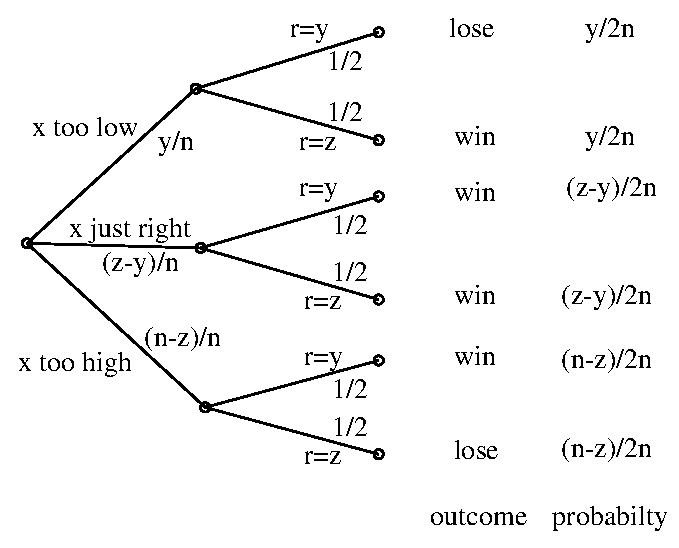
\includegraphics{figures/game100}}}}
  \caption{This is the tree diagram for the Numbers Game.}
  \label{fig:game100}
\end{figure}

%[[[Carl:  There are two typos in this figure.
%``too high'' should be changed to ``just right'', and vice versa.]]]

\emph{Step 1: Find the sample space.} We either choose $x$ too low, too
high, or just right.  Then we either choose $r=y$ or $r=z$.  As
indicated in the figure, this gives a total of six outcomes.

\emph{Step 2: Define events of interest.} We are interested in the
event that we correctly pick the larger number.  This event consists
of four outcomes, which are marked ``win'' in the figure.

\emph{Step 3: Compute outcome probabilities.} As usual, we first assign
probabilities to edges.  First, we guess $x$.  The probability that our
guess of $x$ is too low is $y/n$, the probability that our
guess is too high is $(n-z)/n$, and the probability of a correct
guess is $(z-y)/n$.  We then select an envelope; $r=y$ and $r=z$
occur with equal probability, independent of the choice of $x$.  The
probability of an outcome is the product of the probabilities on the
corresponding root-to-leaf path, as shown in the figure.

\emph{Step 4: Compute event probabilities.} The probability of winning
is the sum of the probabilities of the four winning outcomes.  This
gives:

\begin{eqnarray*}
\pr{\mbox{winning}}
        & = & \frac{y}{2n} + \frac{z-y}{2n} + \frac{z-y}{2n} + \frac{n-z}{2n}\\
        & = & \frac{n + z - y}{2n} \\
        & = & \frac{1}{2} + \frac{z - y}{2n} \\
        & \geq & \frac{1}{2} + \frac{1}{2n}
\end{eqnarray*}

In the final equality, we use the fact that the larger number $z$ is
at least 1 greater than the smaller number $y$, since they must be
distinct.

We conclude that the probability of winning with this strategy is at
least $1/2 + 1/2n$, regardless of the integers in the
envelopes!

For example, if the numbers in the envelopes are in the range $0,
\ldots 100$, then the probability of winning is at least $1/2 +
1/200 = 50.5\%$.  Even better, if the numbers are constrained to
be in the range $0, \ldots, 10$, then the probability of winning rises
to 55\%!  By Las Vegas standards, these are great odds!

\subsubsection{Optimality of the Winning Strategy}

What strategy should our opponent use in putting the numbers into the
envelopes?  That is, how can he ensure that we do not get, say, a 60\%
chance of winning?

Of course, our opponent could try to be clever, putting in two low
numbers and then two high numbers, etc.  But then there is no
guarantee that we will not catch on and start winning every time!

It turns out that our opponent should also use a randomized strategy
involving the uniform distribution.  In particular, he should choose $y$
from $\set{0,\dots n-1}$ uniformly, and then let $z = y+1$.  That is, he
should randomly choose a pair of consecutive integers like $(6,7)$ or
$(73, 74)$ with the uniform distribution.

\begin{claim}\label{clopt}
If the opponent uses the strategy above, then $\pr{\mbox{we win}} \leq
1/2 + 1/2n$ for every strategy we can adopt.
\end{claim}
Claim~\ref{clopt} is not hard to prove once we define just what a
``strategy'' can be, but we won't elaborate that here.  One of consequence
is that both our strategy above of guessing $x$ and the opponent's
strategy above are \emph{optimal}: we can win with probability \emph{at
least} $1/2 + 1/2n$ regardless of what our opponent does, and our opponent
can ensure that we win with probability \emph{at most} $1/2 + 1/2n$
regardless of what we do.

\iffalse THE PRECISE STATEMENT AND PROOF OF THE CLAIM WAS LAST USED IN
SPRING 01 TUT12:

\ppart A \emph{randomized strategy} for you in this game is a function
that, for each number $i$, assigns a probability $p_i$ of switching {\em
given} that the number in the envelope you picked first was $i$.  Prove
that the strategy described in class for winning with probability at least
$1/2 + 1/2n$ is \emph{optimal} for you.  In particular, if David picks $i
\in \Zintvco{0}{n}$ with uniform probability, and then places $i$ and $i+1$ in
each envelope with equal probability, then your probability of winning is
\emph{at most} $1/2 + 1/2n$.

\solution{Let $p_i$ denote the probability that you switch if you see the
number $i$.  Then, the probability that you win if David picks the pair
$(i,i+1)$ is the probability that you will see the smaller number and
switch, or that you will see the bigger number and stay.  Since the
probability of picking either number is $1/2$, the probability that you
win is
\[(1/2)p_i + (1/2)(1-p_{i+1}).
\]
Then the probability that you win is:
\[
\sum_{i=0}^{n-1} \frac{1}{n} \left(\frac{1}{2}p_i + \frac{1}{2}(1-p_{i+1})\right)
= \frac{1}{2} + \frac{1}{2n}\sum_{i=0}^{n-1} (p_i-p_{i+1})
= \frac{1}{2} + \frac{1}{2n} (p_0 - p_n) \leq \frac{1}{2} + \frac{1}{2n}
\]
}
\fi

\iffalse
Spring 01 tut12 also considers the case where our opponent is allowed to
put any non-negative integers into the envelopes; he can use numbers as
large as he likes. This case is more complicated, because the uniform
density on $\nngint$ is not even well-defined.  Nevertheless, there
is a strategy that guarantees a better than 50\% chance of winning
regardless of what numbers are in the envelopes!
\fi

\iffalse

\subsection{Another two-player game}

You remember Monty Hall?  Well, not satisfied with the money 
{\em Let's Make a Deal} is making in syndication, he's turned to 
other sorts of games.  Here's one: 

There are two envelopes, one containing twice as much money as the
other.  He gives you one, but he does not allow you to open it. He
then asks whether you want to keep the envelopes, or switch.
Should you?

Here's some incorrect reasoning: lets say you have $\$x$ in your
current envelope; so with probability $\frac12$ the other envelope has
$\$(2x)$, and with probability $\frac12$ the other envelope has
$\$x/2$.  So your expected gain on swapping is $x/2 - x/4 = x/4$ ---
that is, you should always swap!

But this argument is incorrect, and the reason is that the probability
is not 50-50 that the other envelope has either twice or half as much.
For example, suppose I randomly put \$1 and \$2 in two envelopes.  
You open one and it contains \$2.  What is the probability that
the other envelope contains \$4?  It's zero.

A correct argument, which gives the intuitively reasonable answer
that it makes no difference whether you switch, is the following.
One envelope has $\$y$ and the other has $\$2y$.  So if you open
an envelope and see $\$x$, then either $x = y$ with probability $\frac12$,
or $x = 2y$ with probability $\frac12$.  So in the first case
your gain on switching is $x$, and in the second your gain is $-x$.
Thus your expected gain is zero.

Now Monty allows you to open the envelope in hand, revealing $\$x.$
Again he asks whether you want to keep the money, or switch. Given
this extra information - the actual number $x$ - should you switch or
not. Intuitively, it would seem that knowing the number $x$ does not
give you any edge and so it shouldn't matter whether you switch or
not. But, in actuality there is a strategy which allows you to pick
the larger of the two sums with probability better than $\frac12$. The
strategy is as follows - choose any distribution which has continuous
support over the reals, like the normal distribution, and pick a
number $r$ from it, if $r > x$ then switch, otherwise stay. Note that
whenever $r$ is smaller than the lesser of the two sums or bigger than
the greater of the two then we end up with the larger sum with
probability $\frac12$, but whenever $r$ lies in between the two sums
then we always end up with the larger sum. Thus we do better than
$\frac12$, since there is a non-zero probability of $r$ landing
exactly between the two sums. Note, however, that if we use the normal
distribution to pick $r$ then if the sums in question grow very large
our probability of winning the larger amount goes to $\frac12$. In
fact it can be shown that there is no distribution that can guarantee
us a winning probability greater than $\frac12$ by any fixed constant.
\fi



\subsection{Binomial Distribution Examples}

\subsubsection{The Space Station \emph{Mir}}

The troubled space station \emph{Mir} has $n$ parts, each of which is
faulty with probability $p$.  Assume that faults occur independently, and
let the random variable $R$ be the number of faulty parts.  What is the
probability density of $R$, that is, what is $\pr{R = k}$?  We can answer
this with the usual four-step method, though we will not draw a tree
diagram.

\emph{Step 1: Find the sample space. } We can characterize Mir with a
string of $W$'s and $F$'s of length $n$.  A $W$ in the $i$-th position
indicates that the $i$-th part is working, and an $F$ indicates that
the $i$-th part is faulty.  Each such string is an outcome, and the
sample space $\sspace$ is the set of all $2^n$ such strings.

\emph{Step 2: Define events of interest. } We want to find the
probability that there are exactly $k$ faulty parts; that is, we are
interested in the event that $R = k$.

\emph{Step 3: Compute outcome probabilities. } Since faults occur
independently, the probability of an outcome such as $FWFWW$ is simply
a product such as $p(1-p)p(1-p)(1-p) = p^2(1-p)^3$.  Each $F$
contributes a $p$ term and each $W$ contributes a $(1-p)$ term.  In
general, the probability of an outcome with $k$ faulty parts and $n-k$
working parts is $p^k (1-p)^{n-k}$.

\emph{Step 4: Compute event probabilities. }

We can compute the probability that $k$ parts are faulty as follows:
\begin{eqnarray}
\pr{R = k} & = & \sum_{w \in [R=k]}
              p^k (1-p)^{n-k} \label{Rk.1}\\
& = & \mbox{(\# of length-$n$ strings with $k$ $F$'s)} \cdot p^k (1-p)^{n-k} \label{Rk.2}\\
& = & \binom{n}{k} p^k (1-p)^{n-k}\label{Rk.3}
\end{eqnarray}

Equation~(\ref{Rk.1}) uses the definition of the probability of an event.
Then~(\ref{Rk.2}) follows because all terms in the summation are equal,
and then~(\ref{Rk.3}) follows because there are $\dbinom{n}{k}$ strings of
length $n$ with $k$ occurrrences of $F$.

We can now see that the probability density for the number of faulty parts
is precisely the general binomial density:
\[
f_R(k) \eqdef \pr{R = k} = \binom{n}{k} p^k (1-p)^{n-k} = f_{n, p}(k).
\]
As a sanity check, we should confirm that the sum $\sum_k f_R(k)$ of
these probabilities is one.  This fact follows from the Binomial Theorem:
\[
1 = (p + (1 - p))^n = \sum_{k=0}^n \binom{n}{k}p^k(1-p)^{n-k}.
\]

In general, the binomial distribution arises whenever we have $n$
independent Bernoulli variables with the same distribution.  In this case,
the Bernoulli variables indicated whether a part was faulty or not.  As
another example, if we flip $n$ fair coins, then the number of heads has
an unbiased binomial density.

\subsubsection{Leader Election}

There are $n$ persons in a room. They wish to pick one of themselves as
their leader. They wish to do this in a fair and democratic way, so that
each and everyone has the same chance to be the leader. The scheme they
employ is for everyone to toss a coin. If exactly one person tosses a head
that person is elected the leader. If no persons or more than one person
tosses heads then they repeat the entire process.  

If the coins they use have probability $p$ of coming up heads then
what should $p$ be to maximize the probability of selecting a leader
in a given round? If $n$ coins are tossed then the probability of
having exactly one head is $\dbinom{n}{1} p(1-p)^{n-1}$. Notice that
if $p$ is too large then the likelihood of tossing multiple heads
becomes high, whereas if $p$ is too small then no one tosses a
head. By differentiating the probability with respect to $p$, and then equating
to $0$, we find that the maximum occurs when $p = 1/n$.  Hence, they
should use coins so that the probability of coming up heads is $1/n$.
When they use such coins then the probability of selecting a leader in
a given round is
\[
\binom{n}{1}\frac{1}{n}(1-\frac{1}{n})^{n-1} \sim 1/e.
\]

Leader election is a very common and important idea in distributed
computing. One example is how a set of devices that share a single
communication channel (whether wireless or an ethernet cable) may decide
which device gets to broadcast. If more than one device broadcasts at the
same time, the message will be lost. So the devices keep trying to elect a
leader and when they succeed, the leader gets to broadcast on the
channel.\footnote{Ethernet uses a variant of this idea called \emph{binary
exponential backoff}, where the bias $p$ of the leader election coin is
constantly adjusted because $n$ is unknown. Probabilistic analysis is an
important part of Network theory.} An interesting question is: given some
probability of successfully choosing a leader in a given round, how many
rounds do we expect the devices have to try before they successfully send
a message?  We'll consider this type of question in later Course Notes.


\section{The Shape of the Binomial Distribution}

The binomial distribution is somewhat complicated, and it's hard to see
its qualitative behavior for large $k$ and $n$.

\iffalse

More generally, we would like to know the shape of the binomial
distribution.  That is, what is the value of $f_{n, p}(k)$ for
particular $n$, $p$ and $k$?  Of course, we could simply plug in the
values of these variables, but a simpler, approximate expression would
be nice.

For example, if we flip 100 fair coins, what is the probability that
we get exactly 50 heads?  What is the probability that we get 25 heads
or fewer?

\fi

For example, suppose I flip $100$ coins.  Here are some basic questions we
might ask:
\begin{itemize}
\item what is the most likely number of heads?
\item what the probability of exactly $50$ heads?
\item the probability of exactly $25$ heads?
\item the probability of less than $25$ heads?
\item probability of exactly $25$ heads, given at most $25$?
\end{itemize}

%vote: $1$, $.5$, $.1$, $.01$, $.000001$

To answer these questions, we will develop some closed form approximations
that will help us understand the properties of the binomial density and
cumulative distribution.  Let's first consider the case when the coin is
fair: the \emph{unbiased} density, namely,
\[
f_{n,1/2}(k) \eqdef \binom{n}{k}2^{-n}.
\]

\subsection{The central term}

Where is $f_{n,p}(k)$ maximized?  It's shown in
\href{http://theory.lcs.mit.edu/classes/6.042/spring02/handouts/problemsets/ps9.pdf}
{Spring '02, Problem Set 9} that
\iffalse
\begin{eqnarray*}
f_{n,p}(k)/f_{n.p}(k-1) &=& \frac{n-k+1)p}{k(1-p)}\\
&=& 1+\frac{(n+1)p-k}{k(1-p)}
\end{eqnarray*}
Therefore,
\fi
$f_{n,p}(k)$ increases until $k=p(n+1)$, and decreases after.
So for $p=1/2$, the central term is essentially at $k=n/2$.  Now, by
Stirling's formula we have
\[
\binom{n}{n/2} = \frac{n!}{(n/2)!(n/2)!} \sim 
\frac{\stirling{n}}{\paren{\sqrt{\pi n}\paren{\cfrac{n}{2e}}^{n/2}}^2} =
\sqrt{\frac{2}{\pi n}}2^n.
\]
So 
\begin{equation}\label{unbiased central term}
f_{n,1/2}(n/2) \sim \sqrt{\frac{2}{\pi n}}.
\end{equation}
Note this is an asymptotic bound.  For $n=100$ (our question about coins)
we have $1/\sqrt{50 \pi} \approx 0.079788$, so the probability of
throwing exactly 50 heads in 100 tosses is about 8\%.  In fact, the bound
given above is very close to the true value; in this case, the exact
answer is $0.079589\ldots$.  In general, to determine the accuracy of this
estimate we'll need to use the form of Stirling's formula that gives upper
and lower bounds, which we consider below.

\subsection{The tails}

We can generalize the estimate of the central term at $(1/2)n$ to terms at
factors other than 1/2.  Namely, we estimate $f_{n,1/2}(\alpha n)$ when
$\alpha \neq 1/2$ by first estimating the binomial coefficient
\begin{lemma*}
\begin{equation}\label{binom-est}
\binom{n}{\alpha n} \sim 2^{nH(\alpha)}/\sqrt{2\pi \alpha(1-\alpha)n}
\end{equation}
where
\[
H(\alpha) \eqdef - (\alpha\log_2 \alpha + (1-\alpha)\log_2 (1-\alpha)).
\]
\end{lemma*}
\begin{proof}

\begin{eqnarray*}
\binom{n}{\alpha n} &\eqdef& \frac{n!}{(\alpha n)!((1-\alpha) n)!}\\ 
  &\sim& \frac{\sqrt{2\pi n}\left(\cfrac{n}{e}\right)^n}
         {\sqrt{2\pi \alpha n}\left(\cfrac{\alpha n}{e}\right)^{\alpha n}
          \sqrt{2\pi (1-\alpha) n}\left(\cfrac{(1-\alpha) n}{e}\right)^{(1-\alpha)n}}\\
&=& \left(\frac{1}{\alpha^\alpha(1-\alpha)^{(1-\alpha)}}\right)^n/\sqrt{2\pi \alpha(1-\alpha)n} \\
 &=&     2^{-(\alpha\log_2 \alpha+(1-\alpha)\log_2 (1-\alpha))n}/\sqrt{2\pi \alpha(1-\alpha)n} \\
  &=& 2^{nH(\alpha)}/\sqrt{2\pi \alpha(1-\alpha)n}.
\end{eqnarray*}
\end{proof}

$H(\alpha)$ is the known as the \emph{entropy function}.  Its graph is
shown in Figure~\ref{entropy}.  It is only defined for $0 \le \alpha \le
1$, and takes values between 0 and 1 with its maximum at $H(1/2) = 1$.
The entropy function plays an important role in thermodynamics and in
information theory.

                                % GNUPLOT: LaTeX picture
\begin{figure}
\setlength{\unitlength}{0.240900pt}
\ifx\plotpoint\undefined\newsavebox{\plotpoint}\fi
\sbox{\plotpoint}{\rule[-0.200pt]{0.400pt}{0.400pt}}%
\begin{picture}(1500,900)(0,0)
  \font\gnuplot=cmr10 at 10pt
  \gnuplot
  \sbox{\plotpoint}{\rule[-0.200pt]{0.400pt}{0.400pt}}%
  \put(220.0,113.0){\rule[-0.200pt]{292.934pt}{0.400pt}}
  \put(220.0,113.0){\rule[-0.200pt]{0.400pt}{184.048pt}}
  \put(220.0,113.0){\rule[-0.200pt]{4.818pt}{0.400pt}}
  \put(198,113){\makebox(0,0)[r]{0}}
  \put(1416.0,113.0){\rule[-0.200pt]{4.818pt}{0.400pt}}
  \put(220.0,266.0){\rule[-0.200pt]{4.818pt}{0.400pt}}
  \put(198,266){\makebox(0,0)[r]{0.2}}
  \put(1416.0,266.0){\rule[-0.200pt]{4.818pt}{0.400pt}}
  \put(220.0,419.0){\rule[-0.200pt]{4.818pt}{0.400pt}}
  \put(198,419){\makebox(0,0)[r]{0.4}}
  \put(1416.0,419.0){\rule[-0.200pt]{4.818pt}{0.400pt}}
  \put(220.0,571.0){\rule[-0.200pt]{4.818pt}{0.400pt}}
  \put(198,571){\makebox(0,0)[r]{0.6}}
  \put(1416.0,571.0){\rule[-0.200pt]{4.818pt}{0.400pt}}
  \put(220.0,724.0){\rule[-0.200pt]{4.818pt}{0.400pt}}
  \put(198,724){\makebox(0,0)[r]{0.8}}
  \put(1416.0,724.0){\rule[-0.200pt]{4.818pt}{0.400pt}}
  \put(220.0,877.0){\rule[-0.200pt]{4.818pt}{0.400pt}}
  \put(198,877){\makebox(0,0)[r]{1}}
  \put(1416.0,877.0){\rule[-0.200pt]{4.818pt}{0.400pt}}
  \put(220.0,113.0){\rule[-0.200pt]{0.400pt}{4.818pt}}
  \put(220,68){\makebox(0,0){0}}
  \put(220.0,857.0){\rule[-0.200pt]{0.400pt}{4.818pt}}
  \put(463.0,113.0){\rule[-0.200pt]{0.400pt}{4.818pt}}
  \put(463,68){\makebox(0,0){0.2}}
  \put(463.0,857.0){\rule[-0.200pt]{0.400pt}{4.818pt}}
  \put(706.0,113.0){\rule[-0.200pt]{0.400pt}{4.818pt}}
  \put(706,68){\makebox(0,0){0.4}}
  \put(706.0,857.0){\rule[-0.200pt]{0.400pt}{4.818pt}}
  \put(950.0,113.0){\rule[-0.200pt]{0.400pt}{4.818pt}}
  \put(950,68){\makebox(0,0){0.6}}
  \put(950.0,857.0){\rule[-0.200pt]{0.400pt}{4.818pt}}
  \put(1193.0,113.0){\rule[-0.200pt]{0.400pt}{4.818pt}}
  \put(1193,68){\makebox(0,0){0.8}}
  \put(1193.0,857.0){\rule[-0.200pt]{0.400pt}{4.818pt}}
  \put(1436.0,113.0){\rule[-0.200pt]{0.400pt}{4.818pt}}
  \put(1436,68){\makebox(0,0){1}}
  \put(1436.0,857.0){\rule[-0.200pt]{0.400pt}{4.818pt}}
  \put(220.0,113.0){\rule[-0.200pt]{292.934pt}{0.400pt}}
  \put(1436.0,113.0){\rule[-0.200pt]{0.400pt}{184.048pt}}
  \put(220.0,877.0){\rule[-0.200pt]{292.934pt}{0.400pt}}
  \put(45,495){\makebox(0,0){$H(\alpha)$}}
  \put(828,23){\makebox(0,0){$\alpha$}}
  \put(220.0,113.0){\rule[-0.200pt]{0.400pt}{184.048pt}}
  \put(232,175){\usebox{\plotpoint}}
  \multiput(232.58,175.00)(0.493,1.845){23}{\rule{0.119pt}{1.546pt}}
  \multiput(231.17,175.00)(13.000,43.791){2}{\rule{0.400pt}{0.773pt}}
  \multiput(245.58,222.00)(0.492,1.746){21}{\rule{0.119pt}{1.467pt}}
  \multiput(244.17,222.00)(12.000,37.956){2}{\rule{0.400pt}{0.733pt}}
  \multiput(257.58,263.00)(0.492,1.573){21}{\rule{0.119pt}{1.333pt}}
  \multiput(256.17,263.00)(12.000,34.233){2}{\rule{0.400pt}{0.667pt}}
  \multiput(269.58,300.00)(0.492,1.401){21}{\rule{0.119pt}{1.200pt}}
  \multiput(268.17,300.00)(12.000,30.509){2}{\rule{0.400pt}{0.600pt}}
  \multiput(281.58,333.00)(0.493,1.250){23}{\rule{0.119pt}{1.085pt}}
  \multiput(280.17,333.00)(13.000,29.749){2}{\rule{0.400pt}{0.542pt}}
  \multiput(294.58,365.00)(0.492,1.272){21}{\rule{0.119pt}{1.100pt}}
  \multiput(293.17,365.00)(12.000,27.717){2}{\rule{0.400pt}{0.550pt}}
  \multiput(306.58,395.00)(0.492,1.142){21}{\rule{0.119pt}{1.000pt}}
  \multiput(305.17,395.00)(12.000,24.924){2}{\rule{0.400pt}{0.500pt}}
  \multiput(318.58,422.00)(0.493,1.052){23}{\rule{0.119pt}{0.931pt}}
  \multiput(317.17,422.00)(13.000,25.068){2}{\rule{0.400pt}{0.465pt}}
  \multiput(331.58,449.00)(0.492,1.056){21}{\rule{0.119pt}{0.933pt}}
  \multiput(330.17,449.00)(12.000,23.063){2}{\rule{0.400pt}{0.467pt}}
  \multiput(343.58,474.00)(0.492,0.970){21}{\rule{0.119pt}{0.867pt}}
  \multiput(342.17,474.00)(12.000,21.201){2}{\rule{0.400pt}{0.433pt}}
  \multiput(355.58,497.00)(0.492,0.970){21}{\rule{0.119pt}{0.867pt}}
  \multiput(354.17,497.00)(12.000,21.201){2}{\rule{0.400pt}{0.433pt}}
  \multiput(367.58,520.00)(0.493,0.853){23}{\rule{0.119pt}{0.777pt}}
  \multiput(366.17,520.00)(13.000,20.387){2}{\rule{0.400pt}{0.388pt}}
  \multiput(380.58,542.00)(0.492,0.841){21}{\rule{0.119pt}{0.767pt}}
  \multiput(379.17,542.00)(12.000,18.409){2}{\rule{0.400pt}{0.383pt}}
  \multiput(392.58,562.00)(0.492,0.841){21}{\rule{0.119pt}{0.767pt}}
  \multiput(391.17,562.00)(12.000,18.409){2}{\rule{0.400pt}{0.383pt}}
  \multiput(404.58,582.00)(0.493,0.734){23}{\rule{0.119pt}{0.685pt}}
  \multiput(403.17,582.00)(13.000,17.579){2}{\rule{0.400pt}{0.342pt}}
  \multiput(417.58,601.00)(0.492,0.712){21}{\rule{0.119pt}{0.667pt}}
  \multiput(416.17,601.00)(12.000,15.616){2}{\rule{0.400pt}{0.333pt}}
  \multiput(429.58,618.00)(0.492,0.755){21}{\rule{0.119pt}{0.700pt}}
  \multiput(428.17,618.00)(12.000,16.547){2}{\rule{0.400pt}{0.350pt}}
  \multiput(441.58,636.00)(0.492,0.669){21}{\rule{0.119pt}{0.633pt}}
  \multiput(440.17,636.00)(12.000,14.685){2}{\rule{0.400pt}{0.317pt}}
  \multiput(453.58,652.00)(0.493,0.616){23}{\rule{0.119pt}{0.592pt}}
  \multiput(452.17,652.00)(13.000,14.771){2}{\rule{0.400pt}{0.296pt}}
  \multiput(466.58,668.00)(0.492,0.625){21}{\rule{0.119pt}{0.600pt}}
  \multiput(465.17,668.00)(12.000,13.755){2}{\rule{0.400pt}{0.300pt}}
  \multiput(478.58,683.00)(0.492,0.582){21}{\rule{0.119pt}{0.567pt}}
  \multiput(477.17,683.00)(12.000,12.824){2}{\rule{0.400pt}{0.283pt}}
  \multiput(490.00,697.58)(0.497,0.493){23}{\rule{0.500pt}{0.119pt}}
  \multiput(490.00,696.17)(11.962,13.000){2}{\rule{0.250pt}{0.400pt}}
  \multiput(503.58,710.00)(0.492,0.539){21}{\rule{0.119pt}{0.533pt}}
  \multiput(502.17,710.00)(12.000,11.893){2}{\rule{0.400pt}{0.267pt}}
  \multiput(515.58,723.00)(0.492,0.539){21}{\rule{0.119pt}{0.533pt}}
  \multiput(514.17,723.00)(12.000,11.893){2}{\rule{0.400pt}{0.267pt}}
  \multiput(527.00,736.58)(0.496,0.492){21}{\rule{0.500pt}{0.119pt}}
  \multiput(527.00,735.17)(10.962,12.000){2}{\rule{0.250pt}{0.400pt}}
  \multiput(539.00,748.58)(0.590,0.492){19}{\rule{0.573pt}{0.118pt}}
  \multiput(539.00,747.17)(11.811,11.000){2}{\rule{0.286pt}{0.400pt}}
  \multiput(552.00,759.58)(0.600,0.491){17}{\rule{0.580pt}{0.118pt}}
  \multiput(552.00,758.17)(10.796,10.000){2}{\rule{0.290pt}{0.400pt}}
  \multiput(564.00,769.58)(0.543,0.492){19}{\rule{0.536pt}{0.118pt}}
  \multiput(564.00,768.17)(10.887,11.000){2}{\rule{0.268pt}{0.400pt}}
  \multiput(576.00,780.59)(0.669,0.489){15}{\rule{0.633pt}{0.118pt}}
  \multiput(576.00,779.17)(10.685,9.000){2}{\rule{0.317pt}{0.400pt}}
  \multiput(588.00,789.59)(0.728,0.489){15}{\rule{0.678pt}{0.118pt}}
  \multiput(588.00,788.17)(11.593,9.000){2}{\rule{0.339pt}{0.400pt}}
  \multiput(601.00,798.59)(0.669,0.489){15}{\rule{0.633pt}{0.118pt}}
  \multiput(601.00,797.17)(10.685,9.000){2}{\rule{0.317pt}{0.400pt}}
  \multiput(613.00,807.59)(0.758,0.488){13}{\rule{0.700pt}{0.117pt}}
  \multiput(613.00,806.17)(10.547,8.000){2}{\rule{0.350pt}{0.400pt}}
  \multiput(625.00,815.59)(0.950,0.485){11}{\rule{0.843pt}{0.117pt}}
  \multiput(625.00,814.17)(11.251,7.000){2}{\rule{0.421pt}{0.400pt}}
  \multiput(638.00,822.59)(0.874,0.485){11}{\rule{0.786pt}{0.117pt}}
  \multiput(638.00,821.17)(10.369,7.000){2}{\rule{0.393pt}{0.400pt}}
  \multiput(650.00,829.59)(1.033,0.482){9}{\rule{0.900pt}{0.116pt}}
  \multiput(650.00,828.17)(10.132,6.000){2}{\rule{0.450pt}{0.400pt}}
  \multiput(662.00,835.59)(1.033,0.482){9}{\rule{0.900pt}{0.116pt}}
  \multiput(662.00,834.17)(10.132,6.000){2}{\rule{0.450pt}{0.400pt}}
  \multiput(674.00,841.59)(1.123,0.482){9}{\rule{0.967pt}{0.116pt}}
  \multiput(674.00,840.17)(10.994,6.000){2}{\rule{0.483pt}{0.400pt}}
  \multiput(687.00,847.59)(1.267,0.477){7}{\rule{1.060pt}{0.115pt}}
  \multiput(687.00,846.17)(9.800,5.000){2}{\rule{0.530pt}{0.400pt}}
  \multiput(699.00,852.59)(1.267,0.477){7}{\rule{1.060pt}{0.115pt}}
  \multiput(699.00,851.17)(9.800,5.000){2}{\rule{0.530pt}{0.400pt}}
  \multiput(711.00,857.60)(1.797,0.468){5}{\rule{1.400pt}{0.113pt}}
  \multiput(711.00,856.17)(10.094,4.000){2}{\rule{0.700pt}{0.400pt}}
  \multiput(724.00,861.61)(2.472,0.447){3}{\rule{1.700pt}{0.108pt}}
  \multiput(724.00,860.17)(8.472,3.000){2}{\rule{0.850pt}{0.400pt}}
  \multiput(736.00,864.61)(2.472,0.447){3}{\rule{1.700pt}{0.108pt}}
  \multiput(736.00,863.17)(8.472,3.000){2}{\rule{0.850pt}{0.400pt}}
  \multiput(748.00,867.61)(2.472,0.447){3}{\rule{1.700pt}{0.108pt}}
  \multiput(748.00,866.17)(8.472,3.000){2}{\rule{0.850pt}{0.400pt}}
  \put(760,870.17){\rule{2.700pt}{0.400pt}}
  \multiput(760.00,869.17)(7.396,2.000){2}{\rule{1.350pt}{0.400pt}}
  \put(773,872.17){\rule{2.500pt}{0.400pt}}
  \multiput(773.00,871.17)(6.811,2.000){2}{\rule{1.250pt}{0.400pt}}
  \put(785,874.17){\rule{2.500pt}{0.400pt}}
  \multiput(785.00,873.17)(6.811,2.000){2}{\rule{1.250pt}{0.400pt}}
  \put(810,875.67){\rule{2.891pt}{0.400pt}}
  \multiput(810.00,875.17)(6.000,1.000){2}{\rule{1.445pt}{0.400pt}}
  \put(797.0,876.0){\rule[-0.200pt]{3.132pt}{0.400pt}}
  \put(834,875.67){\rule{2.891pt}{0.400pt}}
  \multiput(834.00,876.17)(6.000,-1.000){2}{\rule{1.445pt}{0.400pt}}
  \put(822.0,877.0){\rule[-0.200pt]{2.891pt}{0.400pt}}
  \put(859,874.17){\rule{2.500pt}{0.400pt}}
  \multiput(859.00,875.17)(6.811,-2.000){2}{\rule{1.250pt}{0.400pt}}
  \put(871,872.17){\rule{2.500pt}{0.400pt}}
  \multiput(871.00,873.17)(6.811,-2.000){2}{\rule{1.250pt}{0.400pt}}
  \put(883,870.17){\rule{2.700pt}{0.400pt}}
  \multiput(883.00,871.17)(7.396,-2.000){2}{\rule{1.350pt}{0.400pt}}
  \multiput(896.00,868.95)(2.472,-0.447){3}{\rule{1.700pt}{0.108pt}}
  \multiput(896.00,869.17)(8.472,-3.000){2}{\rule{0.850pt}{0.400pt}}
  \multiput(908.00,865.95)(2.472,-0.447){3}{\rule{1.700pt}{0.108pt}}
  \multiput(908.00,866.17)(8.472,-3.000){2}{\rule{0.850pt}{0.400pt}}
  \multiput(920.00,862.95)(2.472,-0.447){3}{\rule{1.700pt}{0.108pt}}
  \multiput(920.00,863.17)(8.472,-3.000){2}{\rule{0.850pt}{0.400pt}}
  \multiput(932.00,859.94)(1.797,-0.468){5}{\rule{1.400pt}{0.113pt}}
  \multiput(932.00,860.17)(10.094,-4.000){2}{\rule{0.700pt}{0.400pt}}
  \multiput(945.00,855.93)(1.267,-0.477){7}{\rule{1.060pt}{0.115pt}}
  \multiput(945.00,856.17)(9.800,-5.000){2}{\rule{0.530pt}{0.400pt}}
  \multiput(957.00,850.93)(1.267,-0.477){7}{\rule{1.060pt}{0.115pt}}
  \multiput(957.00,851.17)(9.800,-5.000){2}{\rule{0.530pt}{0.400pt}}
  \multiput(969.00,845.93)(1.123,-0.482){9}{\rule{0.967pt}{0.116pt}}
  \multiput(969.00,846.17)(10.994,-6.000){2}{\rule{0.483pt}{0.400pt}}
  \multiput(982.00,839.93)(1.033,-0.482){9}{\rule{0.900pt}{0.116pt}}
  \multiput(982.00,840.17)(10.132,-6.000){2}{\rule{0.450pt}{0.400pt}}
  \multiput(994.00,833.93)(1.033,-0.482){9}{\rule{0.900pt}{0.116pt}}
  \multiput(994.00,834.17)(10.132,-6.000){2}{\rule{0.450pt}{0.400pt}}
  \multiput(1006.00,827.93)(0.874,-0.485){11}{\rule{0.786pt}{0.117pt}}
  \multiput(1006.00,828.17)(10.369,-7.000){2}{\rule{0.393pt}{0.400pt}}
  \multiput(1018.00,820.93)(0.950,-0.485){11}{\rule{0.843pt}{0.117pt}}
  \multiput(1018.00,821.17)(11.251,-7.000){2}{\rule{0.421pt}{0.400pt}}
  \multiput(1031.00,813.93)(0.758,-0.488){13}{\rule{0.700pt}{0.117pt}}
  \multiput(1031.00,814.17)(10.547,-8.000){2}{\rule{0.350pt}{0.400pt}}
  \multiput(1043.00,805.93)(0.669,-0.489){15}{\rule{0.633pt}{0.118pt}}
  \multiput(1043.00,806.17)(10.685,-9.000){2}{\rule{0.317pt}{0.400pt}}
  \multiput(1055.00,796.93)(0.728,-0.489){15}{\rule{0.678pt}{0.118pt}}
  \multiput(1055.00,797.17)(11.593,-9.000){2}{\rule{0.339pt}{0.400pt}}
  \multiput(1068.00,787.93)(0.669,-0.489){15}{\rule{0.633pt}{0.118pt}}
  \multiput(1068.00,788.17)(10.685,-9.000){2}{\rule{0.317pt}{0.400pt}}
  \multiput(1080.00,778.92)(0.543,-0.492){19}{\rule{0.536pt}{0.118pt}}
  \multiput(1080.00,779.17)(10.887,-11.000){2}{\rule{0.268pt}{0.400pt}}
  \multiput(1092.00,767.92)(0.600,-0.491){17}{\rule{0.580pt}{0.118pt}}
  \multiput(1092.00,768.17)(10.796,-10.000){2}{\rule{0.290pt}{0.400pt}}
  \multiput(1104.00,757.92)(0.590,-0.492){19}{\rule{0.573pt}{0.118pt}}
  \multiput(1104.00,758.17)(11.811,-11.000){2}{\rule{0.286pt}{0.400pt}}
  \multiput(1117.00,746.92)(0.496,-0.492){21}{\rule{0.500pt}{0.119pt}}
  \multiput(1117.00,747.17)(10.962,-12.000){2}{\rule{0.250pt}{0.400pt}}
  \multiput(1129.58,733.79)(0.492,-0.539){21}{\rule{0.119pt}{0.533pt}}
  \multiput(1128.17,734.89)(12.000,-11.893){2}{\rule{0.400pt}{0.267pt}}
  \multiput(1141.58,720.79)(0.492,-0.539){21}{\rule{0.119pt}{0.533pt}}
  \multiput(1140.17,721.89)(12.000,-11.893){2}{\rule{0.400pt}{0.267pt}}
  \multiput(1153.00,708.92)(0.497,-0.493){23}{\rule{0.500pt}{0.119pt}}
  \multiput(1153.00,709.17)(11.962,-13.000){2}{\rule{0.250pt}{0.400pt}}
  \multiput(1166.58,694.65)(0.492,-0.582){21}{\rule{0.119pt}{0.567pt}}
  \multiput(1165.17,695.82)(12.000,-12.824){2}{\rule{0.400pt}{0.283pt}}
  \multiput(1178.58,680.51)(0.492,-0.625){21}{\rule{0.119pt}{0.600pt}}
  \multiput(1177.17,681.75)(12.000,-13.755){2}{\rule{0.400pt}{0.300pt}}
  \multiput(1190.58,665.54)(0.493,-0.616){23}{\rule{0.119pt}{0.592pt}}
  \multiput(1189.17,666.77)(13.000,-14.771){2}{\rule{0.400pt}{0.296pt}}
  \multiput(1203.58,649.37)(0.492,-0.669){21}{\rule{0.119pt}{0.633pt}}
  \multiput(1202.17,650.69)(12.000,-14.685){2}{\rule{0.400pt}{0.317pt}}
  \multiput(1215.58,633.09)(0.492,-0.755){21}{\rule{0.119pt}{0.700pt}}
  \multiput(1214.17,634.55)(12.000,-16.547){2}{\rule{0.400pt}{0.350pt}}
  \multiput(1227.58,615.23)(0.492,-0.712){21}{\rule{0.119pt}{0.667pt}}
  \multiput(1226.17,616.62)(12.000,-15.616){2}{\rule{0.400pt}{0.333pt}}
  \multiput(1239.58,598.16)(0.493,-0.734){23}{\rule{0.119pt}{0.685pt}}
  \multiput(1238.17,599.58)(13.000,-17.579){2}{\rule{0.400pt}{0.342pt}}
  \multiput(1252.58,578.82)(0.492,-0.841){21}{\rule{0.119pt}{0.767pt}}
  \multiput(1251.17,580.41)(12.000,-18.409){2}{\rule{0.400pt}{0.383pt}}
  \multiput(1264.58,558.82)(0.492,-0.841){21}{\rule{0.119pt}{0.767pt}}
  \multiput(1263.17,560.41)(12.000,-18.409){2}{\rule{0.400pt}{0.383pt}}
  \multiput(1276.58,538.77)(0.493,-0.853){23}{\rule{0.119pt}{0.777pt}}
  \multiput(1275.17,540.39)(13.000,-20.387){2}{\rule{0.400pt}{0.388pt}}
  \multiput(1289.58,516.40)(0.492,-0.970){21}{\rule{0.119pt}{0.867pt}}
  \multiput(1288.17,518.20)(12.000,-21.201){2}{\rule{0.400pt}{0.433pt}}
  \multiput(1301.58,493.40)(0.492,-0.970){21}{\rule{0.119pt}{0.867pt}}
  \multiput(1300.17,495.20)(12.000,-21.201){2}{\rule{0.400pt}{0.433pt}}
  \multiput(1313.58,470.13)(0.492,-1.056){21}{\rule{0.119pt}{0.933pt}}
  \multiput(1312.17,472.06)(12.000,-23.063){2}{\rule{0.400pt}{0.467pt}}
  \multiput(1325.58,445.14)(0.493,-1.052){23}{\rule{0.119pt}{0.931pt}}
  \multiput(1324.17,447.07)(13.000,-25.068){2}{\rule{0.400pt}{0.465pt}}
  \multiput(1338.58,417.85)(0.492,-1.142){21}{\rule{0.119pt}{1.000pt}}
  \multiput(1337.17,419.92)(12.000,-24.924){2}{\rule{0.400pt}{0.500pt}}
  \multiput(1350.58,390.43)(0.492,-1.272){21}{\rule{0.119pt}{1.100pt}}
  \multiput(1349.17,392.72)(12.000,-27.717){2}{\rule{0.400pt}{0.550pt}}
  \multiput(1362.58,360.50)(0.493,-1.250){23}{\rule{0.119pt}{1.085pt}}
  \multiput(1361.17,362.75)(13.000,-29.749){2}{\rule{0.400pt}{0.542pt}}
  \multiput(1375.58,328.02)(0.492,-1.401){21}{\rule{0.119pt}{1.200pt}}
  \multiput(1374.17,330.51)(12.000,-30.509){2}{\rule{0.400pt}{0.600pt}}
  \multiput(1387.58,294.47)(0.492,-1.573){21}{\rule{0.119pt}{1.333pt}}
  \multiput(1386.17,297.23)(12.000,-34.233){2}{\rule{0.400pt}{0.667pt}}
  \multiput(1399.58,256.91)(0.492,-1.746){21}{\rule{0.119pt}{1.467pt}}
  \multiput(1398.17,259.96)(12.000,-37.956){2}{\rule{0.400pt}{0.733pt}}
  \multiput(1411.58,215.58)(0.493,-1.845){23}{\rule{0.119pt}{1.546pt}}
  \multiput(1410.17,218.79)(13.000,-43.791){2}{\rule{0.400pt}{0.773pt}}
  \put(846.0,876.0){\rule[-0.200pt]{3.132pt}{0.400pt}}
\end{picture}
\caption{The Entropy Function}\label{entropy}
\end{figure}

For example, the entropy function arises in the study of how much
information is carried in a binary string with a fraction $\alpha$ of the
bits set to one.  Since there are $\dbinom{n}{\alpha n}$ such $n$-bit
strings, they can be numbered using $nH(\alpha) + o(\log n)$-bit binary
numbers.  So the information carried by these $n$-bits can be
``compressed'' into $nH(\alpha)$ bits.  This observation underlies
information-theoretic bounds on the rate at which bits can be reliably
communicated over an unreliable communication channel.

With estimate~(\ref{binom-est}) of the binomial coefficient, we conclude
\begin{equation}\label{unbiased alpha term}
f_{n,1/2}(\alpha n) = \binom{n}{\alpha n}2^{-n} \sim
2^{-n(1 - H(\alpha))}/\sqrt{2\pi \alpha(1-\alpha)n}.
\end{equation}

For $\alpha = 1/2$, this approximation~(\ref{unbiased alpha term}) matches
our estimate~(\ref{unbiased central term}) above.  But now we can also
estimate the probability of throwing exactly 25 heads in 100 tosses.  In
this case, we substitute $n = 100$, and $\alpha = 1/4$ into~(\ref{unbiased
alpha term}) and obtain $1.913 \cdot 10^{-7}$.  The odds are less than 1
in 5 million for throwing exactly 25 heads in 100 tosses!

The estimate in~(\ref{unbiased alpha term}) also provides some important
qualitative understanding of the binomial density.  Note that for
$\alpha \neq 1/2$, we have $1- H(\alpha) > 0$, so
\[
f_{n,1/2}(\alpha n) = O(2^{-\epsilon n})
\]
for $ 1 - H(\alpha) > \epsilon > 0$.  In other words, for $\alpha \neq 1/2$,
\begin{center}
\textbf{$f_{n,1/2}(\alpha n)$ is exponentially small in $n$.}
\end{center}
This means that as $n$ increases, the values any fixed fraction
\iffalse $\alpha - 1/2$ \fi
away from $n/2$ rapidly become less likely, and the likely values
concentrate more and more tightly around $n/2$.

\iffalse

\begin{example}

\[
\binom{n}{n/4} \sim \sqrt{\frac{8}{3\pi n}}2^{0.811n}
\]

$$ f_{n,1/2}(n/4) \sim \sqrt{\frac{8}{3\pi n}}2^{-0.189n} \;\;
\text{exponetially small} $$

Returning to our beginning questions, 
$$ Pr[\mbox{25 heads}] = f_{100,1/2}(25) \approx 1.88 \times 10^{-7} $$

\end{example}

\subsection{Cumulative Distribution}
The {\em cumulative distribution function} $F_R$ of a random variable
$R$, is
\[
F_R(a) \eqdef \pr{R \le a}.
\]

Since $f_{n,1/2}(k)$ is increasing with $k<n/2$, we can bound the
probability $F_R(25) \le 25\cdot f_{n,1/2}(25)$.  But we can do better.

Let $k = \alpha n$ where $\alpha \le 1/2$. Then
%\begin{align*}
%Pr[R\leq \alpha n]
%  &= \sum_{i=0}^{\alpha n} Pr[R=i] \\
%  &= \frac{1}{2^n}\left[ \binom{n}{\alpha n}+\binom{n}{\alpha n - 1}
%  \cdots \binom{n}{0} \right]
%\end{align*}
\begin{eqnarray*}
Pr[R\leq \alpha n]
  &=& \sum_{i=0}^{\alpha n} Pr[R=i] \\
  &=& \frac{1}{2^n}\left[ \binom{n}{\alpha n}+\binom{n}{\alpha n - 1}
  \cdots \binom{n}{0} \right]
\end{eqnarray*}

The term in brackets we can bound by a geometric series by looking
at the ratio of consecutive terms:
%\begin{align*}
%\frac{\binom{n}{r-1}}{\binom{n}{r}} &=
%\frac{\frac{n!}{(r-1)!(n-r+1)!}}{\frac{n!}{r!(n-r)!}}\\
%&= \frac{r}{n-r+1}\\
%&\leq \frac{\alpha n}{n- \alpha n + 1}\\
%&\leq \frac{\alpha}{1-\alpha} \\
%\intertext{
%(Note that we used $r \leq \alpha n$.)
%Therefore,}
%\binom{n}{\alpha n - r} &\le
%\left(\frac{\alpha}{1-\alpha}\right)^r\binom{n}{\alpha n}
%\end{align*}
\begin{eqnarray*}
\frac{\binom{n}{r-1}}{\binom{n}{r}} &=&
\frac{\frac{n!}{(r-1)!(n-r+1)!}}{\frac{n!}{r!(n-r)!}}\\
&=& \frac{r}{n-r+1}\\
&\leq& \frac{\alpha n}{n- \alpha n + 1}\\
&\leq& \frac{\alpha}{1-\alpha}
\end{eqnarray*}
(Note that we used $r \leq \alpha n$.)
Therefore,
\[
\binom{n}{\alpha n - r} \le
\left(\frac{\alpha}{1-\alpha}\right)^r\binom{n}{\alpha n}
\]

Plugging in, we find
%\begin{align*}
%Pr[R\leq \alpha n]
%  &\leq 2^{-n}\left[ \binom{n}{\alpha n} +
%  \frac{\alpha}{1-\alpha}\binom{n}{\alpha n} +
%  \left(\frac{\alpha}{1-\alpha}\right)^2\binom{n}{\alpha n}+ \cdots
%    + \left(\frac{\alpha}{1-\alpha}\right)^{\alpha n}\binom{n}{\alpha
%      n} \right] \\
%    &\leq 2^{-n}\binom{n}{\alpha n}\frac{1}{1-\frac{\alpha}{1-\alpha}}
%    \;\; (\alpha < 1/2 \Rightarrow \frac{\alpha}{1-\alpha}<1) \\
%    &= 2^{-n}\binom{n}{\alpha n}\frac{1-\alpha}{1-2\alpha}
%\end{align*}
\begin{eqnarray*}
Pr[R\leq \alpha n]
  &\leq& 2^{-n}\left[ \binom{n}{\alpha n} +
  \frac{\alpha}{1-\alpha}\binom{n}{\alpha n} +
  \left(\frac{\alpha}{1-\alpha}\right)^2\binom{n}{\alpha n}+ \cdots
    + \left(\frac{\alpha}{1-\alpha}\right)^{\alpha n}\binom{n}{\alpha
      n} \right] \\
    &\leq& 2^{-n}\binom{n}{\alpha n}\frac{1}{1-\frac{\alpha}{1-\alpha}}
    \;\; (\alpha < 1/2 \Rightarrow \frac{\alpha}{1-\alpha}<1) \\
    &=& 2^{-n}\binom{n}{\alpha n}\frac{1-\alpha}{1-2\alpha}
\end{eqnarray*}

Notice that $\frac{1-\alpha}{1-2\alpha}$ is constant!
$$ Pr[\leq 25\mbox{ heads}] \; (n=100, \alpha=1/4) \; = (1.88\times
10^{-7})\frac{3/4}{1/2}  $$

For $\beta = o(\sqrt{n}), f(n/2-\beta\sqrt{n}) \sim \sqrt{\frac{2}{\pi
    n}}e^{-2\beta^2}$.

Furthermore,
%\begin{align*}
%\Pr[\le 24\mbox{ heads}] &\le \frac{\alpha}{1-\alpha}\Pr[\le 25\mbox{
%  heads}]\\
%\intertext{so that}
%\Pr[\mbox{exactly $25$ heads } \mid \mbox{at most $25$ heads}] &> 1/2
%\end{align*}
\[
\Pr[\le 24\mbox{ heads}] \le \frac{\alpha}{1-\alpha}\Pr[\le 25\mbox{
  heads}]
\]
so that
\[
\Pr[\mbox{exactly $25$ heads } \mid \mbox{at most $25$ heads}] > 1/2
\]
\fi

To handle the general case, we define a generalized entropy function
\[
H(\alpha,p) \eqdef - (\alpha \log_2 p + (1 - \alpha) \log_2 (1 - p)).
\]
Then a Stirling formula calculation like the ones above yields
\begin{equation}\label{biased alpha term}
f_{n,p}(\alpha n) = 2^{-n(H(\alpha,p) - H(\alpha))}\overbrace{e^{a_n -
a_{\alpha n} - a_{(1-\alpha) n}}}^{\sim 1}/\sqrt{2 \pi \alpha (1 - \alpha) n}
\end{equation}
The $a_n$ symbols arise from the error in Stirling's approximation; $a_n$
denotes a value between $1/(12n+1)$ and $1/12n$.

The important properties of $H(\alpha,p)$ are:
\begin{align}
H(\alpha, \alpha) & = H(\alpha), & \text{(the ordinary entropy function)} \label{al1}\\
H(\alpha, p) & >  H(\alpha)\geq 0, & \text{ for } 0 < p <1, 0 \leq \alpha
\leq 1, p \neq \alpha \label{al2}\\
H(\alpha, 1/2) & =  1 \label{al3}.
\end{align}

We observed that the maximum value of $f_{n, p}(\alpha n)$ occurs when
$\alpha = p$.  For example, in the Mir problem, each part is faulty with
probability $p$, so we would expect $p n$ faulty parts to be the likeliest
case.  Substituting $\alpha = p$ into~(\ref{biased alpha
term}) and then using equation~(\ref{al1}) gives:
\[
f_{n,p}(pn) \leq \frac{1}{\sqrt{2 \pi p (1-p) n}}.
\]
The two sides of this inequality are actually asymptotically equal.

As in the unbiased case, the main term in our approximation~(\ref{biased
alpha term}) of $f_{n, p}(\alpha n)$ is the power of 2.  If $p = \alpha$,
then $H(p,\alpha)=H(\alpha)$ and the exponent is 0.  However, if $p \neq
\alpha$, then by equation~(\ref{al2}), this term is of the form $2^{-cn}$
for $c = H(\alpha, p) - H(\alpha) > 0$.  Again, this tells us that as $n$
grows large, $f_{n,p}(\alpha n)$ shrinks exponentially, indicating that
the values any fixed fraction \iffalse , $\alpha - 1/2$, \fi away from
$pn$ rapidly become less likely, and the likely values concentrate more
and more tightly around $pn$.  That is, the general binomial density peaks
more and more sharply around $pn$ and has the shape shown in
Figure~\ref{fig:binom}.

\begin{figure}
%\centerline{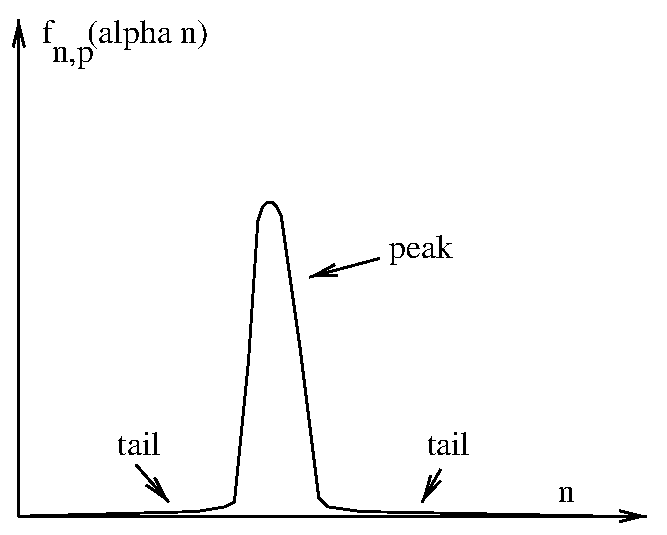
\includegraphics[height=2.5in]{figures/binom}}
  \centerline{\resizebox{!}{2.5in}{\mbox{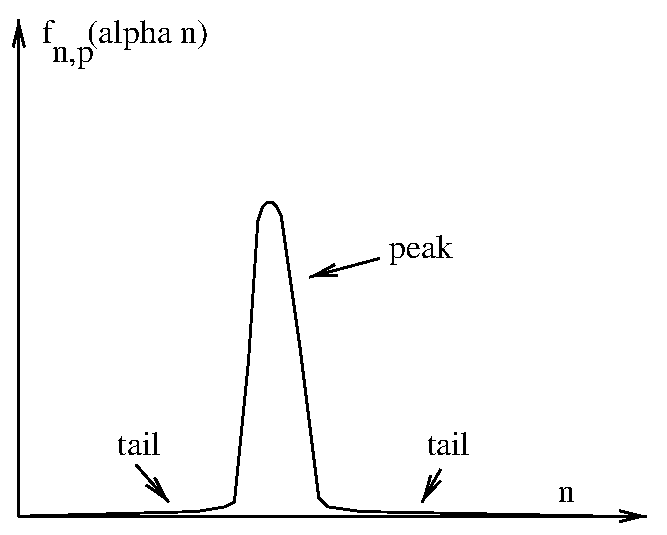
\includegraphics{figures/binom}}}}
  \caption{This diagram shows the approximate shape of the binomial
    density function $f_{n,p}(\alpha n)$.  The horizontal axis goes from
    0 to $n$.  The central peak is
    centered at $\alpha = p$ and has height
    $\Theta(1/\sqrt{n})$ and width
    $\Theta(\sqrt{n})$.  The ``tails'' on either side fall off very
    quickly.}
  \label{fig:binom}
\end{figure}

\iffalse

In fact, as $n \rightarrow \infty$, the density $f_{n,p}$ approaches the
``Bell curve'' or ``normal density.''  Figure~\ref{norm} is a plot of the
normal density in the unbiased case,

                                % GNUPLOT: LaTeX picture
\begin{figure}
\setlength{\unitlength}{0.240900pt}
\ifx\plotpoint\undefined\newsavebox{\plotpoint}\fi
\sbox{\plotpoint}{\rule[-0.200pt]{0.400pt}{0.400pt}}%
\begin{picture}(1500,900)(0,0)
  \font\gnuplot=cmr10 at 10pt
  \gnuplot
  \sbox{\plotpoint}{\rule[-0.200pt]{0.400pt}{0.400pt}}%
  \put(176.0,68.0){\rule[-0.200pt]{303.534pt}{0.400pt}}
  \put(806.0,68.0){\rule[-0.200pt]{0.400pt}{194.888pt}}
  \put(176,68){\usebox{\plotpoint}}
  \put(240,67.67){\rule{2.891pt}{0.400pt}}
  \multiput(240.00,67.17)(6.000,1.000){2}{\rule{1.445pt}{0.400pt}}
  \put(176.0,68.0){\rule[-0.200pt]{15.418pt}{0.400pt}}
  \put(278,68.67){\rule{3.132pt}{0.400pt}}
  \multiput(278.00,68.17)(6.500,1.000){2}{\rule{1.566pt}{0.400pt}}
  \put(291,69.67){\rule{2.891pt}{0.400pt}}
  \multiput(291.00,69.17)(6.000,1.000){2}{\rule{1.445pt}{0.400pt}}
  \put(252.0,69.0){\rule[-0.200pt]{6.263pt}{0.400pt}}
  \put(316,71.17){\rule{2.700pt}{0.400pt}}
  \multiput(316.00,70.17)(7.396,2.000){2}{\rule{1.350pt}{0.400pt}}
  \put(329,72.67){\rule{2.891pt}{0.400pt}}
  \multiput(329.00,72.17)(6.000,1.000){2}{\rule{1.445pt}{0.400pt}}
  \put(341,74.17){\rule{2.700pt}{0.400pt}}
  \multiput(341.00,73.17)(7.396,2.000){2}{\rule{1.350pt}{0.400pt}}
  \put(354,76.17){\rule{2.700pt}{0.400pt}}
  \multiput(354.00,75.17)(7.396,2.000){2}{\rule{1.350pt}{0.400pt}}
  \multiput(367.00,78.61)(2.695,0.447){3}{\rule{1.833pt}{0.108pt}}
  \multiput(367.00,77.17)(9.195,3.000){2}{\rule{0.917pt}{0.400pt}}
  \multiput(380.00,81.60)(1.651,0.468){5}{\rule{1.300pt}{0.113pt}}
  \multiput(380.00,80.17)(9.302,4.000){2}{\rule{0.650pt}{0.400pt}}
  \multiput(392.00,85.60)(1.797,0.468){5}{\rule{1.400pt}{0.113pt}}
  \multiput(392.00,84.17)(10.094,4.000){2}{\rule{0.700pt}{0.400pt}}
  \multiput(405.00,89.59)(1.378,0.477){7}{\rule{1.140pt}{0.115pt}}
  \multiput(405.00,88.17)(10.634,5.000){2}{\rule{0.570pt}{0.400pt}}
  \multiput(418.00,94.59)(0.950,0.485){11}{\rule{0.843pt}{0.117pt}}
  \multiput(418.00,93.17)(11.251,7.000){2}{\rule{0.421pt}{0.400pt}}
  \multiput(431.00,101.59)(0.758,0.488){13}{\rule{0.700pt}{0.117pt}}
  \multiput(431.00,100.17)(10.547,8.000){2}{\rule{0.350pt}{0.400pt}}
  \multiput(443.00,109.59)(0.728,0.489){15}{\rule{0.678pt}{0.118pt}}
  \multiput(443.00,108.17)(11.593,9.000){2}{\rule{0.339pt}{0.400pt}}
  \multiput(456.00,118.58)(0.590,0.492){19}{\rule{0.573pt}{0.118pt}}
  \multiput(456.00,117.17)(11.811,11.000){2}{\rule{0.286pt}{0.400pt}}
  \multiput(469.58,129.00)(0.492,0.539){21}{\rule{0.119pt}{0.533pt}}
  \multiput(468.17,129.00)(12.000,11.893){2}{\rule{0.400pt}{0.267pt}}
  \multiput(481.58,142.00)(0.493,0.576){23}{\rule{0.119pt}{0.562pt}}
  \multiput(480.17,142.00)(13.000,13.834){2}{\rule{0.400pt}{0.281pt}}
  \multiput(494.58,157.00)(0.493,0.655){23}{\rule{0.119pt}{0.623pt}}
  \multiput(493.17,157.00)(13.000,15.707){2}{\rule{0.400pt}{0.312pt}}
  \multiput(507.58,174.00)(0.493,0.774){23}{\rule{0.119pt}{0.715pt}}
  \multiput(506.17,174.00)(13.000,18.515){2}{\rule{0.400pt}{0.358pt}}
  \multiput(520.58,194.00)(0.492,0.927){21}{\rule{0.119pt}{0.833pt}}
  \multiput(519.17,194.00)(12.000,20.270){2}{\rule{0.400pt}{0.417pt}}
  \multiput(532.58,216.00)(0.493,0.972){23}{\rule{0.119pt}{0.869pt}}
  \multiput(531.17,216.00)(13.000,23.196){2}{\rule{0.400pt}{0.435pt}}
  \multiput(545.58,241.00)(0.493,1.052){23}{\rule{0.119pt}{0.931pt}}
  \multiput(544.17,241.00)(13.000,25.068){2}{\rule{0.400pt}{0.465pt}}
  \multiput(558.58,268.00)(0.493,1.171){23}{\rule{0.119pt}{1.023pt}}
  \multiput(557.17,268.00)(13.000,27.877){2}{\rule{0.400pt}{0.512pt}}
  \multiput(571.58,298.00)(0.492,1.401){21}{\rule{0.119pt}{1.200pt}}
  \multiput(570.17,298.00)(12.000,30.509){2}{\rule{0.400pt}{0.600pt}}
  \multiput(583.58,331.00)(0.493,1.369){23}{\rule{0.119pt}{1.177pt}}
  \multiput(582.17,331.00)(13.000,32.557){2}{\rule{0.400pt}{0.588pt}}
  \multiput(596.58,366.00)(0.493,1.448){23}{\rule{0.119pt}{1.238pt}}
  \multiput(595.17,366.00)(13.000,34.430){2}{\rule{0.400pt}{0.619pt}}
  \multiput(609.58,403.00)(0.492,1.659){21}{\rule{0.119pt}{1.400pt}}
  \multiput(608.17,403.00)(12.000,36.094){2}{\rule{0.400pt}{0.700pt}}
  \multiput(621.58,442.00)(0.493,1.607){23}{\rule{0.119pt}{1.362pt}}
  \multiput(620.17,442.00)(13.000,38.174){2}{\rule{0.400pt}{0.681pt}}
  \multiput(634.58,483.00)(0.493,1.607){23}{\rule{0.119pt}{1.362pt}}
  \multiput(633.17,483.00)(13.000,38.174){2}{\rule{0.400pt}{0.681pt}}
  \multiput(647.58,524.00)(0.493,1.646){23}{\rule{0.119pt}{1.392pt}}
  \multiput(646.17,524.00)(13.000,39.110){2}{\rule{0.400pt}{0.696pt}}
  \multiput(660.58,566.00)(0.492,1.789){21}{\rule{0.119pt}{1.500pt}}
  \multiput(659.17,566.00)(12.000,38.887){2}{\rule{0.400pt}{0.750pt}}
  \multiput(672.58,608.00)(0.493,1.607){23}{\rule{0.119pt}{1.362pt}}
  \multiput(671.17,608.00)(13.000,38.174){2}{\rule{0.400pt}{0.681pt}}
  \multiput(685.58,649.00)(0.493,1.567){23}{\rule{0.119pt}{1.331pt}}
  \multiput(684.17,649.00)(13.000,37.238){2}{\rule{0.400pt}{0.665pt}}
  \multiput(698.58,689.00)(0.493,1.488){23}{\rule{0.119pt}{1.269pt}}
  \multiput(697.17,689.00)(13.000,35.366){2}{\rule{0.400pt}{0.635pt}}
  \multiput(711.58,727.00)(0.492,1.444){21}{\rule{0.119pt}{1.233pt}}
  \multiput(710.17,727.00)(12.000,31.440){2}{\rule{0.400pt}{0.617pt}}
  \multiput(723.58,761.00)(0.493,1.250){23}{\rule{0.119pt}{1.085pt}}
  \multiput(722.17,761.00)(13.000,29.749){2}{\rule{0.400pt}{0.542pt}}
  \multiput(736.58,793.00)(0.493,1.052){23}{\rule{0.119pt}{0.931pt}}
  \multiput(735.17,793.00)(13.000,25.068){2}{\rule{0.400pt}{0.465pt}}
  \multiput(749.58,820.00)(0.492,0.927){21}{\rule{0.119pt}{0.833pt}}
  \multiput(748.17,820.00)(12.000,20.270){2}{\rule{0.400pt}{0.417pt}}
  \multiput(761.58,842.00)(0.493,0.655){23}{\rule{0.119pt}{0.623pt}}
  \multiput(760.17,842.00)(13.000,15.707){2}{\rule{0.400pt}{0.312pt}}
  \multiput(774.00,859.58)(0.539,0.492){21}{\rule{0.533pt}{0.119pt}}
  \multiput(774.00,858.17)(11.893,12.000){2}{\rule{0.267pt}{0.400pt}}
  \multiput(787.00,871.59)(1.123,0.482){9}{\rule{0.967pt}{0.116pt}}
  \multiput(787.00,870.17)(10.994,6.000){2}{\rule{0.483pt}{0.400pt}}
  \put(303.0,71.0){\rule[-0.200pt]{3.132pt}{0.400pt}}
  \multiput(812.00,875.93)(1.123,-0.482){9}{\rule{0.967pt}{0.116pt}}
  \multiput(812.00,876.17)(10.994,-6.000){2}{\rule{0.483pt}{0.400pt}}
  \multiput(825.00,869.92)(0.539,-0.492){21}{\rule{0.533pt}{0.119pt}}
  \multiput(825.00,870.17)(11.893,-12.000){2}{\rule{0.267pt}{0.400pt}}
  \multiput(838.58,856.41)(0.493,-0.655){23}{\rule{0.119pt}{0.623pt}}
  \multiput(837.17,857.71)(13.000,-15.707){2}{\rule{0.400pt}{0.312pt}}
  \multiput(851.58,838.54)(0.492,-0.927){21}{\rule{0.119pt}{0.833pt}}
  \multiput(850.17,840.27)(12.000,-20.270){2}{\rule{0.400pt}{0.417pt}}
  \multiput(863.58,816.14)(0.493,-1.052){23}{\rule{0.119pt}{0.931pt}}
  \multiput(862.17,818.07)(13.000,-25.068){2}{\rule{0.400pt}{0.465pt}}
  \multiput(876.58,788.50)(0.493,-1.250){23}{\rule{0.119pt}{1.085pt}}
  \multiput(875.17,790.75)(13.000,-29.749){2}{\rule{0.400pt}{0.542pt}}
  \multiput(889.58,755.88)(0.492,-1.444){21}{\rule{0.119pt}{1.233pt}}
  \multiput(888.17,758.44)(12.000,-31.440){2}{\rule{0.400pt}{0.617pt}}
  \multiput(901.58,721.73)(0.493,-1.488){23}{\rule{0.119pt}{1.269pt}}
  \multiput(900.17,724.37)(13.000,-35.366){2}{\rule{0.400pt}{0.635pt}}
  \multiput(914.58,683.48)(0.493,-1.567){23}{\rule{0.119pt}{1.331pt}}
  \multiput(913.17,686.24)(13.000,-37.238){2}{\rule{0.400pt}{0.665pt}}
  \multiput(927.58,643.35)(0.493,-1.607){23}{\rule{0.119pt}{1.362pt}}
  \multiput(926.17,646.17)(13.000,-38.174){2}{\rule{0.400pt}{0.681pt}}
  \multiput(940.58,601.77)(0.492,-1.789){21}{\rule{0.119pt}{1.500pt}}
  \multiput(939.17,604.89)(12.000,-38.887){2}{\rule{0.400pt}{0.750pt}}
  \multiput(952.58,560.22)(0.493,-1.646){23}{\rule{0.119pt}{1.392pt}}
  \multiput(951.17,563.11)(13.000,-39.110){2}{\rule{0.400pt}{0.696pt}}
  \multiput(965.58,518.35)(0.493,-1.607){23}{\rule{0.119pt}{1.362pt}}
  \multiput(964.17,521.17)(13.000,-38.174){2}{\rule{0.400pt}{0.681pt}}
  \multiput(978.58,477.35)(0.493,-1.607){23}{\rule{0.119pt}{1.362pt}}
  \multiput(977.17,480.17)(13.000,-38.174){2}{\rule{0.400pt}{0.681pt}}
  \multiput(991.58,436.19)(0.492,-1.659){21}{\rule{0.119pt}{1.400pt}}
  \multiput(990.17,439.09)(12.000,-36.094){2}{\rule{0.400pt}{0.700pt}}
  \multiput(1003.58,397.86)(0.493,-1.448){23}{\rule{0.119pt}{1.238pt}}
  \multiput(1002.17,400.43)(13.000,-34.430){2}{\rule{0.400pt}{0.619pt}}
  \multiput(1016.58,361.11)(0.493,-1.369){23}{\rule{0.119pt}{1.177pt}}
  \multiput(1015.17,363.56)(13.000,-32.557){2}{\rule{0.400pt}{0.588pt}}
  \multiput(1029.58,326.02)(0.492,-1.401){21}{\rule{0.119pt}{1.200pt}}
  \multiput(1028.17,328.51)(12.000,-30.509){2}{\rule{0.400pt}{0.600pt}}
  \multiput(1041.58,293.75)(0.493,-1.171){23}{\rule{0.119pt}{1.023pt}}
  \multiput(1040.17,295.88)(13.000,-27.877){2}{\rule{0.400pt}{0.512pt}}
  \multiput(1054.58,264.14)(0.493,-1.052){23}{\rule{0.119pt}{0.931pt}}
  \multiput(1053.17,266.07)(13.000,-25.068){2}{\rule{0.400pt}{0.465pt}}
  \multiput(1067.58,237.39)(0.493,-0.972){23}{\rule{0.119pt}{0.869pt}}
  \multiput(1066.17,239.20)(13.000,-23.196){2}{\rule{0.400pt}{0.435pt}}
  \multiput(1080.58,212.54)(0.492,-0.927){21}{\rule{0.119pt}{0.833pt}}
  \multiput(1079.17,214.27)(12.000,-20.270){2}{\rule{0.400pt}{0.417pt}}
  \multiput(1092.58,191.03)(0.493,-0.774){23}{\rule{0.119pt}{0.715pt}}
  \multiput(1091.17,192.52)(13.000,-18.515){2}{\rule{0.400pt}{0.358pt}}
  \multiput(1105.58,171.41)(0.493,-0.655){23}{\rule{0.119pt}{0.623pt}}
  \multiput(1104.17,172.71)(13.000,-15.707){2}{\rule{0.400pt}{0.312pt}}
  \multiput(1118.58,154.67)(0.493,-0.576){23}{\rule{0.119pt}{0.562pt}}
  \multiput(1117.17,155.83)(13.000,-13.834){2}{\rule{0.400pt}{0.281pt}}
  \multiput(1131.58,139.79)(0.492,-0.539){21}{\rule{0.119pt}{0.533pt}}
  \multiput(1130.17,140.89)(12.000,-11.893){2}{\rule{0.400pt}{0.267pt}}
  \multiput(1143.00,127.92)(0.590,-0.492){19}{\rule{0.573pt}{0.118pt}}
  \multiput(1143.00,128.17)(11.811,-11.000){2}{\rule{0.286pt}{0.400pt}}
  \multiput(1156.00,116.93)(0.728,-0.489){15}{\rule{0.678pt}{0.118pt}}
  \multiput(1156.00,117.17)(11.593,-9.000){2}{\rule{0.339pt}{0.400pt}}
  \multiput(1169.00,107.93)(0.758,-0.488){13}{\rule{0.700pt}{0.117pt}}
  \multiput(1169.00,108.17)(10.547,-8.000){2}{\rule{0.350pt}{0.400pt}}
  \multiput(1181.00,99.93)(0.950,-0.485){11}{\rule{0.843pt}{0.117pt}}
  \multiput(1181.00,100.17)(11.251,-7.000){2}{\rule{0.421pt}{0.400pt}}
  \multiput(1194.00,92.93)(1.378,-0.477){7}{\rule{1.140pt}{0.115pt}}
  \multiput(1194.00,93.17)(10.634,-5.000){2}{\rule{0.570pt}{0.400pt}}
  \multiput(1207.00,87.94)(1.797,-0.468){5}{\rule{1.400pt}{0.113pt}}
  \multiput(1207.00,88.17)(10.094,-4.000){2}{\rule{0.700pt}{0.400pt}}
  \multiput(1220.00,83.94)(1.651,-0.468){5}{\rule{1.300pt}{0.113pt}}
  \multiput(1220.00,84.17)(9.302,-4.000){2}{\rule{0.650pt}{0.400pt}}
  \multiput(1232.00,79.95)(2.695,-0.447){3}{\rule{1.833pt}{0.108pt}}
  \multiput(1232.00,80.17)(9.195,-3.000){2}{\rule{0.917pt}{0.400pt}}
  \put(1245,76.17){\rule{2.700pt}{0.400pt}}
  \multiput(1245.00,77.17)(7.396,-2.000){2}{\rule{1.350pt}{0.400pt}}
  \put(1258,74.17){\rule{2.700pt}{0.400pt}}
  \multiput(1258.00,75.17)(7.396,-2.000){2}{\rule{1.350pt}{0.400pt}}
  \put(1271,72.67){\rule{2.891pt}{0.400pt}}
  \multiput(1271.00,73.17)(6.000,-1.000){2}{\rule{1.445pt}{0.400pt}}
  \put(1283,71.17){\rule{2.700pt}{0.400pt}}
  \multiput(1283.00,72.17)(7.396,-2.000){2}{\rule{1.350pt}{0.400pt}}
  \put(800.0,877.0){\rule[-0.200pt]{2.891pt}{0.400pt}}
  \put(1309,69.67){\rule{2.891pt}{0.400pt}}
  \multiput(1309.00,70.17)(6.000,-1.000){2}{\rule{1.445pt}{0.400pt}}
  \put(1321,68.67){\rule{3.132pt}{0.400pt}}
  \multiput(1321.00,69.17)(6.500,-1.000){2}{\rule{1.566pt}{0.400pt}}
  \put(1296.0,71.0){\rule[-0.200pt]{3.132pt}{0.400pt}}
  \put(1360,67.67){\rule{2.891pt}{0.400pt}}
  \multiput(1360.00,68.17)(6.000,-1.000){2}{\rule{1.445pt}{0.400pt}}
  \put(1334.0,69.0){\rule[-0.200pt]{6.263pt}{0.400pt}}
  \put(1372.0,68.0){\rule[-0.200pt]{15.418pt}{0.400pt}}
\end{picture}
\caption{The Unbiased Normal Density Function}\label{norm}
\end{figure}

The approximation of the binomial density by the normal density is least
accurate in the tails, but these are exponentially small anyway.  We'll
discuss the normal density further in later notes.
\fi

\subsection{The Cumulative Distribution Function}

\subsubsection{25 Heads in 100 Tosses}\label{25H}

What is the probability of tossing 25 or fewer heads?  Of course, we could
sum the probability of zero heads, one head, two heads, \dots, and 25
heads.  But there is also a simple formula in terms of the probability
density function.

\begin{lemma*}
\begin{equation}\label{Fbyf}
F_{n, p}(\alpha n) \leq
\left(\frac{1 - \alpha}{1 - \alpha/p}\right) f_{n, p}(\alpha n)
\end{equation}
for $\alpha < p$.
\end{lemma*}

This Lemma can be proved by considering the ratio of successive values of
$f_{n, p}$.  %
\iffalse as in
\href{http://theory.lcs.mit.edu/classes/6.042/spring02/handouts/problemsets/ps9.pdf}
{Problem Set 9}
\fi
The successive ratios from 0 to $pn$ are approximately
constant, so the sum of these values can be bounded by an increasing
geometric series.  We omit the details.

%derivation in fall 96, lect 22

We can now bound the probability of throwing 25 \emph{or fewer} heads by
plugging in the values $n = 100$, $\alpha = 1/4$ and $p = 1/2$.  This
gives:
\begin{equation*}
\pr{\mbox{at most 25 heads}}
   = F_{100, 1/2}(\frac{1}{4} \cdot 100)
   \leq \frac{3/4}{1/2} f_{100, 1/2}(25)
   = \frac{3}{2} \cdot 1.913\ldots \cdot 10^{-7}.
\end{equation*}

In other words, the probability of throwing 25 or fewer heads is at most
1.5 times the probability of throwing exactly 25 heads.  Therefore, we are
at least twice as likely to throw exactly 25 heads as to throw 24 or
fewer!  This is somewhat surprising; the cases of 0 heads, 1 head, 2
heads, $\dots$, 24 heads are \emph{together} less likely than the single
case of 25 heads.  This shows how quickly the tails of the binomial
density function fall off!

\subsubsection{Transmission Across a Noisy Channel}\label{noisy}

Suppose that we are transmitting bits across a noisy channel.  (For
example, say your modem uses a phone line that faintly picks up a
local radio station.)  Suppose we transmit $10,000$ bits, and each
arriving bit is incorrect with probability $0.01$.  Assume that these
errors occur independently.  What is the probability that more than
$2\%$ of the bits are erroneous?

We can solve this problem using our bound~(\ref{Fbyf}) on $F_{n,p}$.
However, one trick is required because of a technicality: this bound only
holds if $\alpha < p$, so we switch to working with \emph{correct} bits
instead of erroneous bits.

\begin{equation*}
\pr{> \mbox{ than 2\% errors}}
    =  \pr{\leq \mbox{ 98\% correct}} 
    =  F_{n, 0.99}(0.98n) 
    \leq  1.98 \frac{2^{-0.005646 \cdot 10,000}}{0.3509 \sqrt{10,000}}
    \leq  2^{-60}
\end{equation*}

The probability that more than 2\% of the bits are erroneous is
incredibly small!  This again demonstrates the extreme improbability
of outcomes on the tails of the binomial density.
\iffalse

\subsubsection{Polling}

Another good example of binomial distributions comes up in polling.
The Gallup polling service reported that on November 10, only 37\% of
American adults thought Louise Woodward was guilty.  Furthermore,
Gallup asserted that since they asked the opinions of 623 adults,
``one can say with 95 percent confidence that the error attributable
to sampling and other random effects is within plus or minus 4
percentage points''.  Can we confirm this claim?

We want to determine the fraction $p$ of Americans who think that
Louise is guilty.  Our plan is to sample the opinion of $n$ people
chosen uniformly and at random, {\em with replacement}.  That is, we
might poll the same person twice!  This may seem inefficient, but it
simplifies the analysis.  If $G$ is the number of people in our sample
that say Louise is guilty, then we will claim that $p$ is about $G/n$.

The problem is that our sample might not be representative.  For
example, maybe everyone in the country outside of North Dakota thinks
Louise is guilty, but by bad luck the sample contained mostly North
Dakotans.  Then our poll would give the wrong answer.

Let $\epsilon$ be the margin of error we can tolerate, and let
$\delta$ be the probability that our result lies outside this margin.
How many people must we poll so that our result is within $\epsilon$
percent of national opinion with probability at least $1-\delta$?  For
example, Gallup claims that for $\epsilon = 0.04$ and $\delta = 0.05$,
polling $623$ people is sufficient.

We can define $\delta$, the probability that our poll is off by more
than the margin of error $\epsilon$, as follows:

\begin{eqnarray*}
\delta  & = &
        \underbrace{\Pr\left(\frac{G}{n} < p - \epsilon\right)}_{
\begin{array}{c}
\mbox{too many in sample} \\
\mbox{say ``not guilty''}
\end{array}}
        + \underbrace{\Pr\left(\frac{G}{n} > p + \epsilon\right)}_{
\begin{array}{c}
\mbox{too many in sample} \\
\mbox{say ``guilty''}
\end{array}} \\
        & = & \pr{G < (p - \epsilon) n} + \pr{G > (p + \epsilon) n}.
\end{eqnarray*}

Each term in the definition of $\delta$ can be evaluated using
bound~(\ref{Fbyf}) on $F_{n,p}$.  In the second term, we must use the same
trick as in the Noisy Channel problem in Section~\ref{noisy} to
ensure that $\alpha < p$.  We observe that
\[
\pr{\frac{G}{n} > p + \epsilon} = \pr{\frac{n - G}{n} < 1 -p - \epsilon},
\]
where $(n - G)/n$ is the fraction of people polled who say that
Louise is not guilty, and $1-p$ is the fraction of all Americans who say
that she is not guilty.  This gives
\begin{equation}\label{Fnpe}
F_{n,p}((p - \epsilon) n) + F_{n,1-p}((1-p-\epsilon) n)
\end{equation}
as an upper bound for $\delta$.

The problem with the bound~(\ref{Fnpe}) is that the expression
contains the fraction $p$ of Americans who think that Louise is
guilty.  This is the number we are trying to determine by polling!
Fortunately, we can bound $\delta$ by using the following fact:
\begin{fact}
For all $\epsilon$, the maximum value of expression~(\ref{Fnpe}) bounding
$\delta$ occurs when $p = 1/2$.
\end{fact}
\iffalse NEEDS EXPLANATION \fi
This implies that to get an upper bound on $\delta$, we can pretend that
half of the people think Louise is guilty.  So we get
\begin{equation}\label{delta bound}
\delta \leq F_{n,\frac{1}{2}}((\frac{1}{2} - \epsilon) n) +
   F_{n,1-\frac{1}{2}}((1-\frac{1}{2}-\epsilon) n)
 = 2 F_{n}((\frac{1}{2} - \epsilon) n).
\end{equation}

Now suppose that we want a margin of error of $4\%$ as Gallup claimed.
Plugging in $\epsilon = 0.04$ into~(\ref{delta bound}) gives:
\begin{equation*}
\delta \leq   2 F_{n}(0.46 n)
 \leq 
2 \cdot 6.75 \cdot \frac{2^{-0.004622\ldots \cdot n}}{1.2492\ldots \sqrt{n}}.
\end{equation*}

We want to poll enough people so that $\delta$ is less than $0.05$.
The easiest way is to plug in values for $n$, the number of people
polled:
\[
\begin{array}{c|l}
\mbox{$n$ = people polled} & \begin{array}{cc}
\mbox{upper bound on} \\
\mbox{probability poll is wrong}
\end{array} \\
\hline
500 &  9.7\% \\
600 &  6.4\% \\
623 &  5.9\% \quad \leftarrow \quad \mbox{Gallup's poll size} \\
650 &  5.3\% \\
662 &  5.0\% \quad \leftarrow \quad \mbox{our poll size} \\
700 &  4.3\% \\
\end{array}
\]

Gallup's poll size and our poll size are pretty close.  By our
calculation, polling 662 people is sufficient to determine public opinion
to within 4\% with confidence of 95\%.  Gallup only polled 623 people,
which by our calculation gives 94.1\% confidence.  We can look at it
another way: by repeating our calculation with $\epsilon = 0.0413$ plugged
into~(\ref{delta bound}), we can verify that Gallup's poll of 623 people
gives 95\% confidence with at most a 4.13\% margin of error.  Since Gallup
is a first-rate professional pollster, we can assume they have made a more
accurate estimate of appropriate poll size than given by our upper bounds.
Still, our approximations are quite good, since 4.13\% is quite close to
Gallup's announced 4\%.

The remarkable point is that the population of the country has no
effect on the poll size!  Whether there are a thousand people or a
billion in the country, polling only a few hundred is sufficient!
\fi

\iffalse

\subsubsection{Summary}
Unbiased $(p=1/2)$ Binomial Distribution: 
\[
f(\frac{n}{2}) \sim \sqrt{\frac{2}{\pi n}} = \Theta(\frac{1}{\sqrt{n}})
\]
\[
f(\alpha n) \sim \sqrt{\frac{2}{\pi n}}\sqrt{\frac{1}{4\alpha(1-\alpha)}}\frac{1}{2^{n(1-H(\alpha))}}
\;\; (\alpha < 1/2)
\]

General $(p \leq 1/2)$ Binomial Distribution:
\[
f(pn) \sim \sqrt{\frac{1}{2 \pi p(1-p)n}} = \Theta(\frac{1}{\sqrt{pn}})
\]
\[
f(\alpha n) \sim \sqrt{\frac{1}{2 \pi \alpha (1-\alpha)
    n}}2^{n(\alpha\log \frac{p}{\alpha} +
  (1-\alpha)\log\frac{p}{1-\alpha})}
\]
\fi

\section{Expected Value}

The \emph{expectation} of a random variable is a central concept in the
study of probability.  It is the average of all possible values of a
random variable, where a value is weighted according to the probability
that it will appear.  The expectation is sometimes also called the
\emph{average}.  It is also called the \emph{expected value} or the
\emph{mean} of the random variable.  These terms are all synonymous.

\subsection{Two Equivalent Definitions}

\begin{definition}\label{defexp1}
The \emph{expectation} $\expect{R}$ of a random variable $R$ on sample
space $\sspace$ is defined as:
\begin{equation}\label{expsum1}
\expect{R} \eqdef \sum_{s \in \sspace} R(s) \cdot \pr{s}.
\end{equation}
\end{definition}

Another equivalent definition is:
\begin{definition}\label{defexp2}
The \emph{expectation} of random variable $R$ is:
\begin{equation}\label{expsum2}
\expect{R} \eqdef \sum_{r \in \range{R}} r \cdot \pr{R = r}.
\end{equation}
\end{definition}

Actually, there is a technicality implicit in both these definitions that
can cause trouble if ignored.  In both series~(\ref{expsum1})
and~(\ref{expsum2}), the order of the terms in the series is not
specified.  This means that the limits of these series are not
well-defined unless the series are \emph{absolutely convergent}, \ie the
sum of the \emph{absolute values} of the terms converges.  For absolutely
convergent series, the order of summation does not matter---the series
converges to the same value, or else always diverges, regardless of the
order in which the terms are summed.

Definition~\ref{defexp2} is equivalent to Definition~\ref{defexp1},
because each can be obtained from the other simply by grouping the terms
in the series that have the same $R$ value.  Regrouping the terms is
justified because the series are supposed to be absolutely convergent.
Namely, letting $r$ take values over $\range{R}$ we have
\begin{align*}
\expect{R} & =  \sum_{s \in \sspace} R(s) \cdot \pr{s}
                 & \text{(Def.~\ref{defexp1})}\\
       & =   \sum_{r} \sum_{s \in [R = r]} R(s)
       \cdot \pr{s} & \text{(reordering terms)}\\
       & =   \sum_{r} \sum_{s \in [R = r]} r
       \cdot \pr{s} \\
       & =   \sum_{r} r \sum_{s \in [R = r]}
       \pr{s} & \text{(factor out constant $r$)}\\
       & =   \sum_{r} r \pr{R = r}. & \text{(Def. of $\pr{[R=r]}$)}
\end{align*}

\iffalse
If the image of a random variable $R$ is not countable, then the
summation above becomes an integral.  We will not deal with this in
6.042.

\emph{Note: In the previous lecture, a random variable was defined as a
function $R : S \to \reals$.  That is, the range of a random variable was
defined to be the real numbers.  In this lecture, we sometimes consider
random variables over a more limited range.  In particular, we often
consider random variables $R : S \to \nngint$.}
\fi

Like other averages, the expected value of a random variable doesn't say
anything about what will happen in one trial.  For example, the
``average'' American mother has 2.1 children, but obviously none of them
has exactly this number.  So we don't expect to see the expected value of
a random variable in one trial.  Remembering that ``expected'' value
really means ``average'' value may reduce confusion about this point.

But over a large number of independent trials, we do expect the values to
average out close to the expected value.  We'll examine this connection
between the average of a large number of independent trials and the
expectation in detail in Course Notes 12.

\subsection{Expected Value of One Die}

Suppose we roll a fair, six-sided die.  Let the random variable $R$ be
the number that comes up.  We can compute the expected value of $R$
directly from the definition of expected value.
Using the second version of the definition:
\begin{eqnarray*}
\expect{R}  & = &   \sum_{i=1}^6 i \cdot \pr{R = i} \\
        & = &   \frac{1}{6} + \frac{2}{6} + \frac{3}{6} +
                \frac{4}{6} + \frac{5}{6} + \frac{6}{6} \\
        & = &   3.5
\end{eqnarray*}

The average value thrown on a fair die is 3.5.  Again, on one trial---a
single die roll---we will never get an outcome closer to the expected
value than 1/2.  But over many die rolls, the values will almost surely
average to a number very close to 3.5.

By itself, the mean of a random variable doesn't say too much about the
distribution of values of the variable.  Random variables with very
different distributions can have the same mean.  For example, a
nonstandard die with half its sides marked 1 and the other half marked 6
will also have expectation 3.5.

\subsection{Expected Value of an Indicator Variable}

The expected value of an indicator random variable for an event is just
the probability of that event.  Namely, let $I_A$ is the indicator random
variable for event $A$, that is, $I_A = 1$ iff $A$ occurs, otherwise $I_A
= 0$.
\begin{lemma}\label{expindic}
If $I_A$ is the indicator random variable for event $A$, then
\[
\expect{I_A} = \pr{A}.
\]
\end{lemma}

\begin{proof}
\begin{align*}
\expect{I_A} & =  1 \cdot \pr{I_A = 1} + 0 \cdot \pr{I_A = 0} & \text{(Def.~\ref{defexp2})} \\
       & = \pr{I_A = 1}\\
       & =  \pr{A}. & \text{(Def. of $I_A$)}
\end{align*}

\end{proof}


\subsection{The Median is Not the Mean}

Expected value, average, and mean are the same thing, but median is
entirely different.  The median is defined below, but only to make the
distinction clear.  After this, we won't make further use of the median.

\begin{definition}
The {\em median} of a random variable $R$ is the unique value $r$ in the
range of $R$ such that $\pr{R < r} \leq 1/2$ and $\pr{R > r} < 1/2$.

\iffalse (In some texts, the $\leq$ and $<$ are swapped in these two
conditions.)\fi

\end{definition}

For example, with an ordinary die, the median thrown value is $4$, which
is not the same as the mean 3.5.  The median and the mean can be very far
apart.  For example, consider a $2n$-sided die, with $n$ 0s and $n$ 100s.
The mean is $50$, and the median is $100$.

\subsection{Modified Carnival Dice}

Let's look at a modified version of Carnival Dice.  The player chooses a
number from 1 to 6.  He then throws three fair and mutually independent
dice.  He wins one dollar for \emph{each} die that matches his number, and
he loses one dollar if no die matches.

This is better than the original game where the player received one
dollar if any die matched, and lost a dollar otherwise.  At first
glance the new game appears to be fair; after all, the player is now
``justly compensated'' if he rolls his number on more than one die.
In fact, there is still another variant of Carnival Dice in which the
payoff is \$2.75 instead of \$3 if all three dice match.  In this
case, the game appears fair except for the lost quarter in the rare
case that all three dice match.  This looks like a tiny, tolerable
edge for the house.

Let's check our intuition by computing the expected profit of the
player in one round of the \$3 variant of Carnival Dice.  Let the
random variable $R$ be the amount of money won or lost by the player
in a round.  We can compute the expected value of $R$ as follows:
\begin{eqnarray*}
\expect{R}  & = &   -1  \cdot \pr{\mbox{0 matches}} +
                     1 \cdot \pr{\mbox{1 match}} +
                     2  \cdot \pr{\mbox{2 matches}} +
                     3 \cdot \pr{\mbox{3 matches}} \\
        & = &   -1 \cdot \left(\frac{5}{6}\right)^3 +
                1 \cdot 3\left(\frac{1}{6}\right)\left(\frac{5}{6}\right)^2+
                2 \cdot 3\left(\frac{1}{6}\right)^2\left(\frac{5}{6}\right)+
                3 \cdot \left(\frac{1}{6}\right)^3 \\
        & = &   \frac{-125 + 75 + 30 + 3}{216} \\
        & = &   \frac{-17}{216}
\end{eqnarray*}

Our intuition was wrong!  Even with a \$3 payoff for three matching
dice, the player can expect to lose $17/216$ of a dollar, or
about 8 cents, in every round.  This is still a horrible game for the
player!

The \$2.75 variant is deceptive.  One is tempted to believe that a
player is shortchanged only a quarter in the rare case that all three
dice match.  This is a tiny amount.  In fact, though, the player loses
this tiny amount {\em in addition} to the comparatively huge 8 cents
per game!

\section{Expectation of Natural Number-valued Variables}

When the codomain of a random variable is $\nngint$, there is an
alternative way to compute the expected value that can be convenient.  We
can compute the expected value of a random variable $R$ by summing terms
of the form $\pr{R > i}$ instead of terms of the form $\pr{R = i}$.
Remember, though, that the theorem only holds if the codomain of $R$ is
$\nngint$!

%%\subsection{The Method}

\begin{theorem}\label{R>i}
If $R$ is a random variable with range $\nngint$, then
\[
\expect{R} = \sum_{i=0}^{\infty} \pr{R > i}.
\]
\end{theorem}

\begin{proof}
We will begin with the right-hand expression and transform it into
$\expect{R}$.  Because $R$ is natural number valued, we can expand $\pr{R
> i}$ into a series:
\[
\pr{R > i} = \pr{R = i+1} + \pr{R = i+2} + \pr{R = i+1} + \cdots.
\]
So,
\begin{eqnarray*}
\sum_{i=0}^{\infty} \pr{R > i}
        & = & \pr{R > 0} + \pr{R > 1} +  \pr{R > 2} + \cdots \\
        & = & \underbrace{\pr{R = 1} +  \pr{R = 2} + \pr{R = 3} + \cdots}_{\pr{R > 0}} \\
        &   & \qquad\qquad\quad
              +\underbrace{\pr{R = 2} + \pr{R = 3} + \cdots}_{\pr{R > 1}} \notag\\
        &   & \qquad\qquad\qquad\qquad\qquad\quad\,
	      +\underbrace{\pr{R = 3} + \cdots}_{\pr{R > 2}} \notag \\
        & = &  \pr{R = 1} + 2 \cdot \pr{R = 2} + 3 \cdot \pr{R = 3} + \cdots \\
        & = &  \sum_{i=0}^{\infty} i \cdot \pr{R = i} \\
        & = &  \expect{R}.
\end{eqnarray*}

\iffalse
In line~(\ref{series}), we rewrite each term $\pr{R > i}$ as a
series;   Next, we sum all the resulting series, and then revert
to $\Sigma$ notation.  The last summation is the definition of
$\expect{R}$.
\fi

\end{proof}

\subsection{Mean Time to Failure}

The Mir space station computer is constantly on the blink.  Fortunately, a
failure is not catastrophic.  Suppose that Mir's main computer has
probability $p$ of failing every hour, and assume that failures occur
independently.  How long should a cosmonaut expect to wait until the main
computer fails?

Let the random variable $R$ be the number of hours until the first
failure; more precisely, assuming that the hours are numbered $1, 2, 3,
\ldots$, then $R$ is the \emph{number of the hour} in which the first
failure occurs.

We want to compute the expected value of $R$.  It turns out to be easy to
compute $\pr{R > i}$, the probability that the first failure occurs
sometime after hour $i$.  Since the range of $R$ is $\nngint$, we can
therefore apply Theorem~\ref{R>i} to compute the expected number of hours.

We can compute $\pr{R > i}$ with the usual four-step method.

{\em Step 1: Find the Sample Space.} We can regard the sample space as a
set of finite strings $W^nF$ for $n \in \nngint$.  A $W$ in the $i$th
position means that the main computer is working during hour $i$.  An $F$
in the $n+1$st position means that the computer went down during hour
$n+1$.

\iffalse
MANY STEPS OMIITED HERE: SHOULD SHOW PROBABILITIES SUM TO 1 AND
THAT FAILURES ARE INDEPENDENT.  WE OUGHT TO DEVELOP A LITTLE THEORY TO
REACH THESE CONCLUSIONS ON GENERAL PRINCIPLE INSTEAD OF BY AD HOC
EVALUATION OF SERIES.
\fi

{\em Step 2: Define Events of Interest.} We are concerned with the
event that $R > i$.  This event consists of all outcomes with no $F$
in the first $i$ positions.

{\em Step 3: Compute Outcome Probabilities.} We want to compute the
probability of a particular outcome $W^nF$.  We reason that since the
probability of a $W$ is $(1-p)$ and of $F$ is $p$, then we shall define
\[
\pr{W^nF} \eqdef (1-p)^np.
\]

{\em Step 4: Compute Event Probabilities.}  We want to compute $\pr{R >
i}$.  There is no $F$ in the first position of an outcome string with
probability $1-p$.  Since failures occur independently, if there is no $F$
in first position, then the probability of $F$ the second position is
$1-p$, etc.  Now we can multiply conditional probabilities: the
probability that there is no $F$ in the first $i$ positions is $(1-p)^i$.
Therefore,
\begin{equation}\label{pR>i}
\pr{R > i} = (1-p)^i.
\end{equation}

Now we have
\begin{align*}
\expect{R}  & = \sum_{i=0}^{\infty} \pr{R > i} & \text{(Thm~\ref{R>i})}\\
   & \sum_{i=0}^{\infty} (1-p)^i \label{fail1} & \text{(by~(\ref{pR>i}))}\\
%        & =   1 + (1-p) + (1-p)^2 + (1-p)^3 + \cdots\\
        & =   \frac{1}{1 - (1-p)} & \text{(sum of geometric series)}\\
        & =   \frac{1}{p}.
\end{align*}

So we have shown that the expected hour when the main computer fails is
$1/p$.  For example, if the computer has a 1\% chance of failing every
hour, then we would expect the first failure to occur at the 100th hour,
or in about four days.  On the bright side, this means that the cosmonaut
can expect 99 comfortable hours {\em without} a computer failure.

%% changed waiting for a boy to waiting for a girl :) (RAD)
%% Seems that Leighton's original notes (97) had girl as well but
%% somewhere along the way this was changed to boy. Just changing it back!

\subsection{Waiting for a Baby Girl}

A couple really wants to have a baby girl.  There is a 50\% chance
that each child they have is a girl, and the genders of their children
are mutually independent.  If the couple insists on having children
until they get a girl, then how many baby boys should they expect
to have first?

This is really a variant of the previous problem.  The question, ``How
many hours until the main computer fails?'' is mathematically the same
as the question, ``How many children must the couple have until they
get a girl?''  In this case, a computer failure corresponds to having
a girl, so we should set $p = 1/2$.  By the preceding analysis, the
couple should expect a baby girl after having $1/p = 2$ children.
Since the last of these will be the girl, they should expect just 1
baby boy.

This strategy may seem to be favoring girls, because the couple keeps
trying until they have one.  However, this effect is counterbalanced
by the small possibility of a long sequence of boys.

Suppose the couple has a $3/4$ chance of having a boy instead of
$1/2$.  Then what is the expected number of children up to and
including the first girl?

Let $R$ be the number of children up to and including the first girl.
Then\[ \expect{R} = \frac{1}{1/4} = 4. \]
That is, the expected number of boys before the first girl is $3$.

\iffalse
{\bf Exercise:} What is the expected number of children needed to get
{\em both} a girl and a boy?
\fi

\section{An Expectation Paradox}

Here is a game that reveals a strange property of expectations.

First, you think of a probability distribution function on the natural
numbers.  This distribution can be absolutely anything you like.  For
example, you might choose a uniform distribution on $1, 2, \ldots, 6$,
giving something like a fair die.  Or you might choose a binomial
distribution on $0, 1, \ldots, n$.  You can even give every natural number
a non-zero probability, provided, of course, that the sum of all
probabilities is 1.  Next, I pick a random number $z$ according to
whatever distribution you invent.  In the final stage, you pick a random
number $y$ according to the same distribution.  If your number is bigger
than mine ($y > z$), then the game ends.  Otherwise, if our numbers are
equal or mine is bigger ($y \leq z$), then you pick again, and keep
picking until you get a value that is bigger than $z$.

What is the expected number of picks that you must make?

Certainly, you always need at least one pick---and one pick won't always
work---so the expected number is greater than one.  An answer like 2 or 3
sounds reasonable, though you might suspect that the answer depends on the
distribution.  The real answer is amazing: the expected number of picks
that you need is always \emph{infinite, regardless of the distribution you
choose!}  This makes sense if you choose, say, the uniform distribution on
$1, 2, \ldots, 6$.  After all, there is a $1/6$ chance that I will pick 6.
In this case, you must pick forever--- you can never beat me!

To calculate the expected number of picks, let's first consider the
probability that you need more than one pick.  By symmetry there is at
least a 50-50 chance that my $z$ is greater than or equal to your $y$, and
you will have to pick again.  In other words, you need more than one pick
with probability at least 1/2.

What is the probability that you need more than two picks?  Here is an
erroneous argument.
\begin{falseproof}
On the first pick, you beat me with probability at most $1/2$.  On the
second pick, you beat me with probability at most $1/2$.  The probability
that you fail to beat me on both picks is at most
\[
\frac{1}{2} \cdot \frac{1}{2} = \frac{1}{4}.
\]
Therefore, the probability that you need more than two picks is at most
1/4.
\end{falseproof}

The problem with this reasoning is that beating me on your second pick is
not independent of beating me on your first pick, so multiplying the
probabilities of these two events isn't valid.  It's going to be harder to
beat me on your second pick: the fact that you are picking a second time
implies that $z$ beat a randomly chosen $y$.  So this means $z$ is likely
to be a harder-than-average number to beat on the next pick.

Here is a correct argument: the probability that you need more than two
picks is the same as the probability that if I pick $z$ and you
independently pick $y_1$ and $y_2$, then $z$ is greater than or equal to
the maximum of $z$, $y_1$ and $y_2$.  But by symmetry, each of these
number choices is as likely as any of the others to equal their maximum.
So the probability that any one of them is equal to their maximum is at
least 1/3---it will actually be even larger than 1/3 because of the
possibility of ties for the maximum.  So in particular, the probabilty
that $z$ is the maximum, and hence that you need more than two picks, is
at least $1/3$.

Similarly, we can see that the probability that you need more than $i$
picks is at least $1/(i+1)$---just replace ``2'' by ``$i$'' and ``3'' by
``$i+1$'' in the previous argument for more than two picks.  So if we let
$T$ be the random variable equal to the number of picks you need to beat
me, then
\begin{equation}\label{T>i}
\pr{T > i} \geq \frac{1}{i+1}.
\end{equation}

This argument also shows your chance of needing more picks will be even
larger when there are ties.  So you should choose a distribution such that
ties are very rare.  For example, you might choose the uniform
distribution on $\set{1,\dots, 10^{100}}$.  In this case, the probability
that you need more than $i$ picks to beat me is very close to $1/(i+1)$
for reasonable $i$.  For example, the probability that you need more than
99 picks is almost exactly 1\%.  This may sound very promising to you;
intuitively, you might expect to win within a reasonable number of picks
on average.  But now we can verify the claim that, contrary to intuition,
the expected number of picks that you need in order to beat me is
infinite.  The proof is simple:

\begin{proof}
\begin{align*}
\expect{T} & =  \sum_{i=0}^{\infty} \pr{T > i} & \text{(Thm.~\ref{R>i})}\\
           & \geq  \sum_{i=0}^{\infty} \frac{1}{i+1} & \text{(by~(\ref{T>i}))}\\
           & =  \infty. & \text{(sum of Harmonic series)}
\end{align*}
\end{proof}

This phenomenon can cause all sorts of confusion.  For example, suppose
we have a communication network.  Assume that a packet has a $1/i$ chance
of being delayed by $i$ or more steps.  This sounds good; there is only a
1\% chance of being delayed by 100 or more steps.  But, by the argument
above, the expected delay for a packet is actually infinite!

\section{Linearity of Expectation}\label{finlin}

\subsection{Expectation of a Sum}

Expected values obey a simple, very helpful rule called
\hyperdef{ln11}{linearity}{\emph{Linearity of Expectation}}.  Its simplest
form says that the expected value of a sum of random variables is the sum
of the expected values of the variables.

\begin{theorem}\label{expsum-2}
For any random variables $R_1$ and $R_2$,
\[
\expect{R_1 + R_2} = \expect{R_1} + \expect{R_2}.
\]
\end{theorem}

\begin{proof}
Let $T \eqdef R_1+R_2$.  The proof follows straightforwardly by
rearranging terms using Definition~\ref{defexp1} of $\expect{T}$.
\begin{align*}
\expect{R_1 + R_2} & \eqdef \expect{T}\\
        & \eqdef \sum_{s \in \sspace} T(s) \cdot \pr{s}
                       & \text{(Def.~\ref{defexp1})}\\
        & = \sum_{s \in \sspace} (R_1(s) + R_2(s)) \cdot \pr{s}
                         & \text{(Def. of $T$)}\\
        & = \sum_{s \in \sspace} R_1(s) \pr{s} + 
              \sum_{s \in \sspace} R_2(s) \pr{s} & \text{(rearanging terms)}\\
        & = \expect{R_1} + \expect{R_2}.  & \text{(Def.~\ref{defexp1})}
\end{align*}
\end{proof}

Similarly, we have
\begin{lemma}\label{constexp}
For any random variable $R$ and constant $a \in \reals$,
\begin{equation*}
\expect{aR} = a\expect{R}.
\end{equation*}
\end{lemma}
The proof follows easily from the definition of expectation, and we omit
it.

Combining Theorem~\ref{expsum-2} and Lemma~\ref{constexp}, we conclude
\begin{theorem}\label{linexp-2-thm}[Linearity of Expectation]
\[
\expect{a_1R_1 + a_2R_2} = a_1\expect{R_1} + a_2\expect{R_2}
\]
for all random variables $R_1,R_2$ and constants $a_1,a_2 \in \reals$.
\end{theorem}
In other words, expectation is a linear function.  The same rule holds
for more than two random variables:
\begin{corollary}\label{linexp-k-thm}
For any random variables $R_1, \dots, R_k$, and constants $a_1, \dots, a_k
\in \reals$,
\[
\expect{\sum_{i=1}^k a_iR_i} = \sum_{i=1}^k a_i\expect{R_i}.
\]
\end{corollary}
Corollary~\ref{linexp-k-thm} follows from Theorem~\ref{linexp-2-thm} by a
routine induction on $k$ which we omit.

The great thing about linearity of expectation is that \emph{no
independence is required}.  This is really useful, because dealing with
independence is a pain, and we often need to work with random variables
that are not independent.

\iffalse Even when the random variables \emph{are} independent, we know
from previous experience that proving independence requires a lot of
work.\fi


\subsection{Expected Value of Two Dice}

What is the expected value of the sum of two fair dice?

Let the random variable $R_1$ be the number on the first die, and let
$R_2$ be the number on the second die.  We observed earlier that the
expected value of one die is 3.5.  We can find the expected value of the
sum using linearity of expectation:
\begin{equation*}
\expect{R_1 + R_2} 
 =   \expect{R_1} + \expect{R_2}
 =    3.5 + 3.5
 =    7.
\end{equation*}

Notice that we did {\em not} have to assume that the two dice were
independent.  The expected sum of two dice is 7, even if they are
glued together!  (This is provided that gluing does not change weights
to make the individual dice unfair.)

Proving that the expected sum is 7 with a tree diagram would be hard;
there are 36 cases.  And if we did not assume that the dice were
independent, the job would be a nightmare!

\subsection{The Hat-Check Problem}

There is a dinner party where $N$ men check their hats.  The hats are
mixed up during dinner, so that afterward each man receives a random
hat.  In particular, each man gets his own hat with probability
$1/N$.  What is the expected number of men who get their own
hat?

Without linearity of expectation, this would be a very difficult
question to answer.  We might try the following.  Let the random
variable $R$ be the number of men that get their own hat.  We want to
compute $\expect{R}$.  By the definition of expectation, we have:
\[
\expect{R} = \sum_{k=0}^{N} k \cdot \pr{R = k}.
\]

Now we are in trouble, because evaluating $\pr{R = k}$ is a mess and
we then need to substitute this mess into a summation.  Furthermore,
to have any hope, we would need to fix the probability of each
permutation of the hats.  For example, we might assume that all
permutations of hats are equally likely.

Now let's try to use linearity of expectation.  As before, let the
random variable $R$ be the number of men that get their own hat.  The
trick is to express $R$ as a sum of indicator variables.  In
particular, let $R_i$ be an indicator for the event that the $i$th
man gets his own hat.  That is, $R_i = 1$ is the event that he gets
his own hat, and $R_i = 0$ is the event that he gets the wrong hat.
The number of men that get their own hat is the sum of these
indicators:
\[
R = R_1 + R_2 + \cdots + R_N.
\]

These indicator variables are {\em not} mutually independent.  For
example, if $N-1$ men all get their own hats, then the last man is
certain to receive his own hat.
\iffalse
That is, if $R_1 = R_2 = \ldots = R_{N-1} = 1$, then we know that $R_N = 1$.
\fi
So $R_N$ is not independent of the other indicator variables.  But, since
we plan to use linearity of expectation, we \emph{don't care} whether the
indicator variables are independent, because no matter what,
we can take the expected value of both sides of the equation above and
apply linearity of expectation:
\begin{equation*}
\expect{R} =  \expect{R_1 + R_2 + \cdots + R_N} 
           =  \expect{R_1} + \expect{R_2} + \cdots + \expect{R_N}.
\end{equation*}
Now by Lemma~\ref{expindic}, the expected value of an indicator variable
is always the probability that the indicator is 1.  In this case, the
quantity $\pr{R_i = 1}$ is the probability that the $i$th man gets his
own hat, which is just $1/N$.  We can now compute the expected number of
men that get their own hat:
\[\begin{array}{rcccccccccc}
\expect{R} &=&  \expect{R_1} &+& \expect{R_2} &+& \cdots &+& \expect{R_N} \\
           &=&  \cfrac{1}{N} &+& \cfrac{1}{N} &+& \cdots &+& \cfrac{1}{N} &=& 1.
\end{array}\]

We should expect exactly one man to get the right hat!

Notice that we did not assume that all permutations of hats are
equally likely or even that all permutations are possible.  We only needed
to know that each man received his own hat with probability
$1/N$.  This makes our solution very general, as the next
example shows.

\subsection{The Chinese Appetizer Problem}

There are $N$ people at a circular table in a Chinese restaurant.  On
the table, there are $N$ different appetizers arranged on a big Lazy
Susan.  Each person starts munching on the appetizer directly in front
of them.  Then someone spins the Lazy Susan so that everyone is faced
with a random appetizer.  What is the expected number of people that
end up with the appetizer that they had originally?

This is just a special case of the hat-check problem, with appetizers in
place of hats.  In the hat check problem, we assumed only that each man
received his own hat with probability $1/N$; we made no assumptions about
how the hats could be permuted.  This problem is a special case, because
we happen to know that appetizers are cyclically shifted relative to their
initial position.  (We assume that each cyclic shift is equally likely.)
Our previous analysis still holds; the expected number of people that get
their original appetizer is one.

Of course the event that exactly one person gets his original appetizer
never happens: either everyone does or no one does.  This is another
example of the important point that the ``expected value'' is not the same
as ``the value we expect,'' since the expected value may never occur!

\subsection{Expected Number of Events that Occur}

We can generalize the hat-check and appetizer problems even further.
Suppose that we have a collection of events in a sample space.  What is
the expected number of events that occur?  For example, $A_i$ might be the
event that the $i$th man receives his own hat.  The number of events that
occur is then the number of men that receive their own hat.  Linearity of
expectation gives a general solution to this problem:

\begin{theorem}
Given any collection of events $A_1, A_2, \dots, A_N$, the expected number
of these events that occur is
\[
\sum_{i=1}^N \pr{A_i}.
\]
\end{theorem}

The theorem says that the expected number of events that occur is the
sum the probabilities of the events.  For example, in the hat-check
problem the probability of the event that the $i$th man receives his
hat is $1/N$.  Since there are $N$ such events, the theorem
says that the expected number of men that receive their hat is $N
(1/N) = 1$.  This matches our earlier result.
No independence assumptions are needed.

The proof follows immediately from Lemma~\ref{expindic} and the fact that
$R$ is the sum of the indicator variables for the $A_i$.
That is,
\[
R = \sum_i I_{A_i},
\]
and
so
\[
\expect{R} = \expect{\sum_i I_{A_i}} = \sum_i \expect{I_{A_i}} = \sum_i \pr{A_i}.
\]

\subsection{Expectation of a Binomial Distribution}

Suppose that we independently flip $n$ biased coins, each with probability
$p$ of coming up heads.  What is the expected number that come up heads?

Let $H_{n,p}$ be the number of heads after the flips.  Then $H_{n,p}$ has
the binomial distribution with parameters $n$ and $p$.  Now let $I_k$ be
the indicator for the $k$th coin coming up heads.  By
Lemma~\ref{expindic}, we have
\[
\expect{I_k} = p.
\]
But
\[
H_{n,p} = \sum_{k=1}^n I_k,
\]
so by linearity
\[
\expect{H_{n,p}} = \expect{\sum_{k=1}^n I_k} = \sum_{k=1}^n \expect{I_k} =
\sum_{k=1}^n p = pn.
\]

That is, the expectation of a $n,p$-binomially distributed variable is
$pn$.

\iffalse

Let $A_i$ be the event that coin $i$ comes up heads.
Since the coin is fair, $\pr{A_i} = 1/2$.  Since
there are $N$ coins in all, there are $N$ such events.  By the theorem
in the last section, the expected number of events that occur (the
number of coins that come up heads) is $N(1/2) =
N/2$.

Let's try to solve the same problem the hard way.  In this case,
assume that the coins are fair.  Let the random variable $R$ be the
number of heads.  We want to compute the expected value of $R$.

\begin{eqnarray*}
\expect{R}  & = & \sum_{i=0}^N i \cdot \pr{R = i} \\
        & = & \sum_{i=0}^N i \binom{N}{i} 2^{-N}
\end{eqnarray*}

The first equation follows from the definition of expectation.  In the
second step, we evaluate $\pr{R = i}$.  An outcome of tossing the $N$
coins can be represented by a length $N$ sequence of $H$'s and $T$'s.
An $H$ in position $i$ indicates that the $i$th coin is heads, and a
$T$ indicates that the $i$th coin is tails.  The sample space
consists of all $2^N$ such sequences.  The outcomes are equiprobable,
and so each has probability $2^{-N}$.  The number of outcomes with
exactly $i$ heads is the number of length $N$ sequences with $i$
$H$'s, which is $\binom{N}{i}$.  Therefore, $\pr{R = i} = \binom{N}{i}
2^{-N}$.

The answer from linearity of expectation and from the hard way must be
the same, so we can equate the two results to obtain a neat identity.

\begin{eqnarray*}
\sum_{i=0}^N i \binom{N}{i} 2^{-N} & = & \frac{N}{2} \\
\sum_{i=0}^N i \binom{N}{i} & = & N2^{N-1}
\end{eqnarray*}

In fact, we proved this identity by another method earlier in the
term.  Note that linearity of expectation solves the problem more
easily and that the result is more general, since we do not need to
assume that the coins are independent.  The expected number of
heads is $N/2$, even if some coins are glued together.


We can extend this reasoning to $n$ tosses of a coin with probability $p$
of a head, rather than 1/2.  If we do this, we get the generalized
combinatorial identity:
\begin{eqnarray*}
\sum_{i=0}^N i \binom{N}{i} p^i (1-p)^{N-i} & = & N p
\end{eqnarray*}
Here, the $p^i$ factor gives the probabilities for the heads and the
$(1-p)^{N-i}$ factor gives the probabilities for the tails.  The
right-hand side is the sum of $N$ terms, each giving the probability
of a particular $A_i$, which is $p$.  The total is $N p$.  For
example, consider an ordinary die.  Let $A_1$ be the event that the
value is odd, $A_2$ the event that the value is $1$, $2$ or $3$, and
$A_3$ the event that the value is $4$, $5$ or $6$.  These events are
not mutually independent.  However, the expected number of these
events that occur is still obtainable by adding $\pr{A_1} + \pr{A_2} +
\pr{A_3}$, which yields 3/2.

{\bf Question:} What can we say about the product of expectations?
For example, can we say $\expect{R_1 R_2} = \expect{R_1}
\expect{R_2}$?  Not in general. We will see more of this in just a
little bit.

\fi

\section{Conditional Expectation}

Just like event probabilities, expectations can be conditioned on some
event.

\begin{definition}\label{defcondexp}
We define \emph{conditional expectation,  $\expcond{R}{A}$, of a random
variable $R$ given event $A$}:
\[
\expcond{R}{A} \eqdef \sum_r r \cdot\prcond{R=r}{A}.
\]
\end{definition}

In other words, it is the expected value of the variable $R$ once we skew
the distribution of $R$ to be conditioned on event $A$.
\begin{example}
Let $D$ be the outcome of a roll of a random fair die.  What is $\expcond{D}{D
\ge 4}$?
\[
\sum_{i=1}^6 i \cdot \prcond{D=i}{D \ge 4} = \sum_{i=4}^6 i \cdot 1/3 = 5
\]
\end{example}

Since $\expcond{R}{A}$ is just an expectation over a different probability
measure, we know that the rules for expectation will extend to conditional
expectation.  For example, conditional expectation will also be linear
\begin{theorem}\label{condexplin}
\[
\expcond{a_1R_1+a_2R_2}{A} = a_1\expcond{R_1}{A} + a_2\expcond{R_2}{A}.
\]
\end{theorem}

A real benefit of conditional expectation is the way it lets us divide
complicated expectation calculations into simpler cases.
\begin{theorem}\label{thm:condexp}[Law of Total Expectation]
If the sample space is the disjoint union of events $A_1,A_2,\cdots$, then
\[
\expect{R} = \sum_i \expcond{R}{A_i} \pr{A_i}.
\]
\end{theorem}

\begin{proof}
  \begin{align*}
    \expect{R} &= \sum_r r \cdot \pr{R=r} & \text{(Def.~\ref{defexp2})}\\
    &= \sum_r r \cdot \sum_i \prcond{R=r}{A_i} \pr{A_i}
            & \text{(Total Probability)}\\
    &= \sum_r \sum_i r \cdot \prcond{R=r}{A_i} \pr{A_i}
              & \text{(distribute constant $r$)}\\
    &= \sum_i \sum_r r \cdot \prcond{R=r}{A_i} \pr{A_i}
              & \text{(exchange order of summation)}\\
    &= \sum_i \pr{A_i} \sum_r r \cdot \prcond{R=r}{A_i}
             & \text{(factor constant $\pr{A_i}$)}\\
    &= \sum_i \pr{A_i} \expcond{R}{A_i}
             & \text{(Def.~\ref{defcondexp})}.
  \end{align*}
\end{proof}

\begin{example}
Half the people in the world are male, half female.  The expected
height of a randomly chosen male is $5'11''$, while the expected
height of a randomly chosen female is $5'5''$.  What is the expected
height of a randomly chosen individual?

Let $H(P)$ be the height of the random person $P$.  The events
$M=$``$P$ is male'' and $F=$``$P$ is female'' are a partition of the
sample space (at least for the moment---though with modern science
you never know).  Then
\begin{align*}
\expect{H} &= \expcond{H}{M} \pr{M} + \expcond{H}{F} \pr{F}\\
&= 5'11'' \cdot \frac12 + 5'5'' \cdot \frac12\\
&= 5'8''
\end{align*}
\end{example}
We will see in the following sections that the Law of Total Expectation
has much more power than one might think.



\section{The Expected Value of a Product}

\subsection{The Product of Independent Expectations}

We have determined that the expectation of a sum is the sum of the
expectations.  The same is not always true for products: in general, the
expectation of a product need \emph{not} equal the product of the
expectations.  But it is true in an important special case, namely, when
the random variables are \emph{independent}.

\begin{theorem}\label{th:prod}
For any two \emph{independent} random variables, $R_1$ and $R_2$,
\[
\expect{R_1 \cdot R_2} = \expect{R_1} \cdot \expect{R_2}.
\]
\end{theorem}

\begin{proof}
We apply the Law of Total Expectation by conditioning on the value
of~$R_1$.
\begin{align*}
\expect{R_1 \cdot R_2} & = \sum_{r \in \range{R_1}} \expcond{R_1 \cdot
           R_2}{R_1 = r} \cdot \pr{R_1 = r} & \text{(Def.~\ref{defcondexp})}\\
   & = \sum_{r} \expcond{r \cdot
           R_2}{R_1 = r} \cdot \pr{R_1 = r}\\
   & = \sum_{r} r \cdot \expcond{R_2}{R_1 = r} \cdot \pr{R_1 = r}
                 & \text{(Thm~\ref{condexplin})}\\
   & = \sum_{r} r \cdot \expect{R_2} \cdot \pr{R_1 = r}
                     & \text{($R_2$ independent of $R_1$)}\\
   & = \expect{R_2} \sum_{r} r \cdot \pr{R_1 = r}
              & \text{(factor out constant $\expect{R_2}$)}\\
  & = \expect{R_2} \cdot \expect{R_1}. & \text{(Def.~\ref{defexp2})}
\end{align*}
\end{proof}

Theorem~\ref{th:prod} extends to a collection of mutually independent
variables.
\begin{corollary}
If random variables $R_1, R_2, \dots, R_k$ are mutually
independent, then
\[
\expect{\prod_{i=1}^k R_i} = \prod_{i=1}^k \expect{R_i}.
\]
\end{corollary}
We omit the simple proof by induction on $k$.

\subsection{The Product of Two Dice}

Suppose we throw two \emph{independent}, fair dice and multiply the
numbers that come up.  What is the expected value of this product?

Let random variables $R_1$ and $R_2$ be the numbers shown on the two
dice.  We can compute the expected value of the product as follows:
\begin{displaymath}\label{R1R2}
  \expect{R_1 \cdot R_2}
  = \expect{R_1} \cdot \expect{R_2}
  = 3.5 \cdot 3.5
  = 12.25.
\end{displaymath}
Here the first equality holds by Theorem~\ref{th:prod} because the dice
are independent.

Now suppose that the two dice are \emph{not} independent; in fact, assume
that the second die is always the same as the first.  In this case, the
product of expectations will not equal the expectation of the product.

To verify this, let random variables $R_1$ and $R_2$ be the numbers shown
on the two dice.  We can compute the expected value of the product without
Theorem~\ref{th:prod} as follows:
\begin{align*}
\expect{R_1 \cdot R_2} & = \expect{R_1^2} & (R_2 = R_1)\\
        & =    \sum_{i=1}^6 i^2 \cdot \pr{R_{1}^2 = i^2}
                    & \text{(Def.~\ref{defexp2})} \\
        & =    \sum_{i=1}^6 i^2 \cdot \pr{R_{1} = i}\\
        & =    \frac{1^2}{6} + \frac{2^2}{6} + \frac{3^2}{6} + 
                \frac{4^2}{6} + \frac{5^2}{6} + \frac{6^2}{6} \\
        & =    15\; \frac{1}{6}\\
        & \neq  12 \; \frac{1}{4}\\
        & = \expect{R_1} \cdot \expect{R_2}. & \text{((\ref{R1R2}))}
\end{align*}


\iffalse
The preceding example shows that for \emph{dependent} variables,
the expected value of a product need not be the product of the
expected values; that is, $\expect{R_1 \cdot R_2} \neq \expect{R_1} \cdot
\expect{R_2}$.

The general rules for expected values of sums and products
are summarized below:

\bigskip

\fbox{\parbox{6.25in}{
\vspace{.25cm}
For random variables $R_1$ and $R_2$:
\begin{itemize}
\item Regardless of whether $R_1$ and $R_2$ are independent,
$\expect{R_1 + R_2} = \expect{R_1} + \expect{R_2}$.
\item If $R_1$ and $R_2$ are independent, then $\expect{R_1 \cdot R_2} =
\expect{R_1} \cdot \expect{R_2}$.
\end{itemize}
}}
\fi

\section{Expectation of a Quotient}

\subsection{A RISC Paradox}

The following data is taken from a paper by some famous professors.  They
wanted to show that programs on a RISC processor are generally shorter
than programs on a CISC processor.  For this purpose, they applied a RISC
compiler and then a CISC compiler to some benchmark source programs and
made a table of compiled program lengths.
\[
\begin{array}{lccc}
\text{Benchmark}        & \text{RISC}   & \text{CISC}   & \text{CISC/RISC}\\
\hline
\text{E-string search}  & 150           & 120           & 0.8 \\
\text{F-bit test}       & 120           & 180           & 1.5 \\
\text{Ackerman}         & 150           & 300           & 2.0 \\
\text{Rec 2-sort}       & 2800          & 1400          & 0.5 \\
\hline
\text{Average}          &               &               & 1.2
\end{array}
\]
Each row contains the data for one benchmark.  The numbers in the second
and third columns are program lengths for each type of compiler.  The
fourth column contains the ratio of the CISC program length to the RISC
program length.  Averaging this ratio over all benchmarks gives the value
1.2 in the lower right.  The authors conclude that ``CISC programs are
20\% longer on average''.

However, some critics of their paper took the same data and argued this
way: redo the final column, taking the other ratio, RISC/CISC instead of
CISC/RISC.
\[
\begin{array}{lccc}
\text{Benchmark}        & \text{RISC}   & \text{CISC}   & \text{RISC/CISC}\\
\hline
\text{E-string search}  & 150           & 120           & 1.25 \\
\text{F-bit test}       & 120           & 180           & 0.67 \\
\text{Ackerman}         & 150           & 300           & 0.5 \\
\text{Rec 2-sort}       & 2800          & 1400          & 2.0 \\
\hline
\text{Average}          &               &               & 1.1
\end{array}
\]
From this table, we would conclude that RISC programs are 10\% longer
than CISC programs on average!  We are using the same reasoning as in
the paper, so this conclusion is equally justifiable--- yet the result
is opposite!  What is going on?

\subsection{A Probabilistic Interpretation}

To resolve these contradictory conclusions, we can model the RISC vs.\ CISC
debate with the machinery of probability theory.

Let the sample space be the set of benchmark programs.  Let the random
variable $R$ be the length of the compiled RISC program, and let the
random variable $C$ be the length of the compiled CISC program.  We would
like to compare the average length $\expect{R}$ of a RISC program to the
average length $\expect{C}$ of a CISC program.

To compare average program lengths, we must assign a probability to
each sample point; in effect, this assigns a ``weight'' to each
benchmark.  One might like to weigh benchmarks based on how frequently
similar programs arise in practice.  Lacking such data, however, we
will assign all benchmarks equal weight; that is, our sample space is
uniform.

In terms of our probability model, the paper computes $C / R$ for each
sample point, and then averages to obtain $\expect{C / R} = 1.2$.  This
much is correct.  The authors then conclude that ``CISC programs are 20\%
longer on average''; that is, they conclude that $\expect{C} = 1.2\,
\expect{R}$.

Similarly, the critics calculation correctly showed that $\expect{R/C} =
1.1$.  They then concluded that $\expect{R} = 1.1 \, \expect{C}$, that is,
a RISC program is 10\% longer than a CISC program on average.

These arguments make a natural assumption, namely, that
\begin{falseclm}\label{false-quotient}
If $S$ and $T$ are independent random variables with $T>0$, then
\[
\expect{\frac{S}{T}} = \frac{\expect{S}}{\expect{T}}.
\]
\end{falseclm}

In other words False Claim~\ref{false-quotient} simply generalizes the
rule for expectation of a product to a rule for the expectation of a
quotient.  But the rule for requires independence, and we surely don't
expect $C$ and $R$ to be independent: large source programs will lead to
large compiled programs, so when the RISC program is large, so the CISC
would be too.

However, we can easily compensate for this kind of dependence: we should
compare the lengths of the programs \emph{relative to the size of the
source code}.  While the lengths of $C$ and $R$ are dependent, it's more
plausible that their \emph{relative} lengths will be independent.  So we
really want to divide the second and third entries in each row of the
table by a ``normalizing factor'' equal to the length of the benchmark
program in the first entry of the row.

But note that normalizing this way will have no effect on the fourth
column!  That's because the normalizing factors applied to the second and
and third entries of the rows will cancel.  So the independence hypothesis
of False Claim~\ref{false-quotient} may be justified, in which case the
authors' conclusions would be justified.  But then, so would the
contradictory conclusions of the critics.  Something must be wrong!  Maybe
it's False Claim~\ref{false-quotient} (duh!), so let's try and prove it.

\begin{falseproof}
\begin{align}
\expect{\frac{S}{T}} & = \expect{S \cdot \frac{1}{T}} \notag\\
       & = \expect{S} \cdot \expect{\frac{1}{T}} & \text{(independence of $S$
       and $T$)}\label{indST}\\
      & = \expect{S} \cdot \frac{1}{\expect{T}}. \label{bug}\\
      & = \frac{\expect{S}}{\expect{T}}.\notag
\end{align}
Note that line~(\ref{indST}) uses the fact that if $S$ and $T$ are
independent, then so are $S$ and $1/T$.  This holds because functions of
independent random variables yield independent random variables, as shown
in
\href{http://theory.lcs.mit.edu/classes/6.042/spring02/handouts/miscellaneous/cp10W.pdf}
{Spring '02 Class Problems 10-1, problem 4}.
\end{falseproof}

But this proof is bogus!  The bug is in line~(\ref{bug}), which assumes
\begin{falsethm}\label{false-inverse}
\[
\expect{\frac{1}{T}} =  \frac{1}{\expect{T}}.
\]
\end{falsethm}
Here is a counterexample:
\begin{example*}
Suppose $T=1$ with probability $1/2$ and $T= 2$ with probability $1/2$.
Then
\begin{eqnarray*}
\frac{1}{\expect{T}} & = &\frac{1}{1 \cdot \frac{1}{2} + 2 \cdot \frac{1}{2}}\\
    & = & \frac{2}{3}\\
    & \neq & \frac{3}{4}\\
    & = &\frac{1}{1} \cdot \frac{1}{2} + \frac{1}{2} \cdot \frac{1}{2}\\
    & = & \expect{\frac{1}{T}}.
\end{eqnarray*}
The two quantities are not equal, so False Claim~\ref{false-inverse}
really is false.
\end{example*}

Unfortunately, the fact that Claim~\ref{false-quotient}
and~\ref{false-inverse} are false does not mean that they are never used!

\subsection{The Proper Quotient}

We can compute $\expect{R}$ and $\expect{C}$ as follows:
\begin{eqnarray*}
\expect{R}  & = &   \sum_{i \in \text{Range(R)}} i \cdot \pr{R = i} \\
        & = &   \frac{150}{4}+\frac{120}{4}+\frac{150}{4}+\frac{2800}{4} \\
        & = &   805 \\
\\
\expect{C}  & = &   \sum_{i \in \text{Range(C)}} i \cdot \pr{C = i} \\
        & = &   \frac{120}{4}+\frac{180}{4}+\frac{300}{4}+\frac{1400}{4} \\
        & = &   500
\end{eqnarray*}

Now since $\expect{R}/\expect{C} = 1.61$, we conclude that the average
RISC program is 61\% longer than the average CISC program.  This is a
third answer, completely different from the other two!  Furthermore, this
answer makes RISC look really bad in terms of code length.  This one is
the correct conclusion, under our assumption that the benchmarks deserve
equal weight.  Neither of the earlier results were correct---not
surprising since both were based on the same false Claim.

\subsection{A Simpler Example [Optional]}

\begin{optional}

The source of the problem is clearer in the following, simpler example.
Suppose the data were as follows.
\[
\begin{array}{lcccc}
\text{Benchmark}        & \text{Processor A}    & \text{Processor B}
                        & B / A                 & A / B  \\
\hline
\text{Problem 1}        & 2                     & 1             
                        & 1/2                   & 2 \\
\text{Problem 2}        & 1                     & 2
                        & 2                     & 1/2 \\
\hline
\text{Average}          &                       &
                        & 1.25                  & 1.25
\end{array}
\]

Now the data for the processors A and B is exactly symmetric; the two
processors are equivalent.  Yet, from the third column we would
conclude that Processor B programs are 25\% longer on average, and
from the fourth column we would conclude that Processor A programs are
25\% longer on average.  Both conclusions are obviously wrong.

The moral is that one must be very careful in summarizing data, we must
not take an average of ratios blindly!

\end{optional}

\section{Infinite Linearity of Expectation}

We know that expectation is linear over finite sums.  It's useful to
extend this result to infinite summations.  This works as long as we avoid
sums whose values may depend on the order of summation.

\subsection{Convergence Conditions for Infinite Linearity}

\begin{theorem}\label{linexp} [Linearity of Expectation]
Let $R_0$, $R_1$, \dots, be random variables such that
\[
\sum_{i = 0}^\infty \expect{\abs{R_i}}
\]
converges.  Then
\[
   \expect{\sum_{i = 0}^\infty R_i} = \sum_{i = 0}^\infty \expect{R_i}.
\]
\end{theorem}

\begin{proof}
Let $T \eqdef \sum_{i = 0}^\infty R_i$.

We leave it to the reader to verify that, under the given convergence
hypothesis, all the sums in the following derivation are absolutely
convergent, which justifies rearranging them as follows:
\begin{align*}
\sum_{i=0}^\infty \expect{R_i}
    &= \sum_{i=0}^\infty \sum_{s \in \sspace} R_i(s) \cdot \prob{s} 
            & \text{(Def.~\ref{defexp1})}\\
    &= \sum_{s \in \sspace} \sum_{i=0}^\infty R_i(s) \cdot \prob{s} 
           & \text{(exchanging order of summation)}\\
    &= \sum_{s \in \sspace} \left[ \sum_{i=0}^\infty R_i(s) \right] \cdot \prob{s}
                & \text{(factoring out $\pr{s}$)}\\
    &= \sum_{s \in \sspace} T(s) \cdot \prob{s} & \text{(Def.\ of $T$)}\\
    &= \expect{T} & \text{(Def.~\ref{defexp1})}\\
    &= \expect{\sum_{i = 0}^\infty R_i}. &  \text{(Def.\ of $T$)}.
\end{align*}
\end{proof}

Note that the finite linearity of expectation we established in
Corollary~\ref{linexp-k-thm} follows as a special case of
Theorem~\ref{linexp}: since $\expect{R_i}$ is finite, so is
$\expect{\abs{R_i}}$, and therefore so is their sum for $0 \leq i \leq n$.
Hence the convergence hypothesis of Theorem~\ref{linexp} is trivially
satisfied if there are only finitely many $R_i$'s.

\iffalse
\textbf{Exercise:} Show that linearity of expectation fails for the sum of
two variables, one with expectation $+\infty$ and the other with
$-\infty$.
\fi

\subsection{A Paradox}
One of the simplest casino bets is on ``red'' or ``black'' at the roulette
table.  In each play at roulette, a small ball is set spinning around a
roulette wheel until it lands in a red, black, or green colored slot.
The payoff for a bet on red or black matches the bet; for example, if you bet
$\$10$ on red and the ball lands in a red slot, you get back your original
$\$10$ bet plus another matching $\$10$.

In the US, a roulette wheel has 2 green slots among 18 black and 18 red
slots, so the probability of red is $p::= 18/38 \approx 0.473$.  In
Europe, where roulette wheels have only 1 green slot, the odds for red
are a little better ---that is, $p = 18/37 \approx 0.486$---but still less
than even.  To make the game fair, we might agree to ignore green, so that
$p = 1/2$.

There is a notorious gambling strategy which seems to guarantee a profit
at roulette: bet $\$10$ on red, and keep doubling the bet until a red
comes up.  This strategy implies that a player will leave the game as a
net winner of $\$10$ as soon as the red first appears.  Of course the
player may need an awfully large bankroll to avoid going bankrupt before
red shows up---but we know that the mean time until a red occurs is $1/p$,
so it seems possible that a moderate bankroll might actually work out.
(In this setting, a ``win'' on red corresponds to a ``failure'' in a
mean-time-to-failure situation.)

Suppose we have the good fortune to gamble against a fair roulette wheel.
In this case, our expected win on any spin is zero, since at the $i$th
spin we are equally likely to win or lose $10 \cdot 2^{i-1}$ dollars.  So
our expected win after any finite number of spins remains zero, and
therefore our expected win using this gambling strategy is zero.  This is
just what we should have anticipated in a fair game.

But wait a minute.  As long as there is a fixed, positive probability of
red appearing on each spin of the wheel---even if the wheel is
unfair---it's \emph{certain} that red will eventually come up.  So with
probability one, we leave the casino having won $\$10$, and our expected
dollar win is obviously $\$10$, not zero!

Something's wrong here.  What?

\subsection{Solution to the Paradox}

The expected amount won is indeed $\$10$.

The argument claiming the expectation is zero is flawed by an invalid use
of linearity of expectation for an infinite sum.  To pinpoint this flaw,
let's first make the sample space explicit: a sample point is a sequence
$B^nR$ representing a run of $n \geq 0$ black spins terminated by a red
spin.  Since the wheel is fair, the probability of $B^nR$ is $2^{-(n+1)}$.

Let $C_i$ be the number of dollars won on the $i$th spin.  So 
$C_i = 10 \cdot 2^{i-1}$ 
when red comes up for the first time on the $i$th spin, that is, at
precisely one sample point, namely $B^{i-1}R$.  Similarly, 
$C_i = -10  \cdot  2^{i-1}$ 
when the first red spin comes up after the $i$th spin, namely, at the
sample points $B^nR$ for $n \geq i$.  Finally, we will define $C_i$ by
convention to be zero at sample points in which the session ends before the
$i$th spin, that is, at points $B^nR$ for $n < i-1$.

The dollar amount won in any gambling session is the value of the sum
$\sum_{i = 1}^\infty C_i$.  At any sample point $B^nR$, the value of this
sum is
\[
10 \cdot -(1 + 2 + 2^2 + \dots + 2^{n - 1}) + 10 \cdot 2^n  = 10,
\]
which trivially implies that its expectation is 10 as well.  That is, the
amount we are \emph{certain} to leave the casino with, as well as
expectation of the amount we win, is $\$10$.

Moreover, our reasoning that $\expect{C_i} = 0$ is sound, so 
\[
\sum_{i = 1}^\infty \expect{C_i} = \sum_{i = 1}^\infty 0 = 0.
\]

The flaw in our argument is the claim that, since the expectation at each
spin was zero, therefore the final expectation would also be zero.
Formally, this corresponds to concluding that
\[
\expect{\mbox{amount won}}  =  \expect{\sum_{i = 1}^\infty C_i}
  =  \sum_{i = 1}^\infty \expect{C_i} = 0.
\]
The flaw lies exactly in the second equality.  This is a case where
linearity of expectation fails to hold---even though both $\sum_{i =
1}^\infty \expect{C_i}$ and $\expect{\sum_{i = 1}^\infty C_i}$ are
finite---because the convergence hypothesis needed for linearity is false.
Namely, the sum
\[
\sum_{i = 1}^\infty \expect{\abs{C_i}}
\]
does not converge.  In fact, the expected value of $\abs{C_i}$ is $10$
because $\abs{C_i} =  10 \cdot 2^{i}$  with probability $2^{-i}$ and
otherwise is zero, so this sum rapidly approaches infinity.

Probability theory truly leads to this apparently paradoxical conclusion: a
game allowing an unbounded---even though always finite---number of ``fair''
moves may not be fair in the end.  In fact, our reasoning leads to an even
more startling conclusion: even against an \emph{unfair} wheel, as long as
there is some fixed positive probability of red on each spin, we are
certain to win $\$10$!

This is clearly a case where naive intuition is unreliable: we don't
expect to beat a fair game, and we do expect to lose when the odds are
against us.  Nevertheless, the ``paradox'' that in fact we always win by
bet-doubling cannot be denied.

But remember that from the start we chose to assume that no one goes
bankrupt while executing our bet-doubling strategy.  This assumption is
crucial, because the expected loss while waiting for the strategy to
produce its ten dollar profit is actually infinite!  So it's not
surprising, after all, that we arrived at an apparently paradoxical
conclusion from an unrealistic assumption.

This example also serves a warning that in making use of infinite
linearity of expectation, the convergence hypothesis which justifies it
had better be checked.


\section{Wald's Theorem}

\subsection{Random Length Sums}

Wald's Theorem concerns the expected sum of a random number of random
variables.  For example, suppose that I flip a coin.  If I get heads, then
I roll two dice.  If I get tails, then I roll three dice.  What is the
expected sum of the dice that I roll?  Wald's Theorem supplies a simple
answer: the average number of dice I roll is 2 1/2, and the average value
of a single die roll is (1+2+\dots+6)/6 = 3 1/2, so the expected sum is (2
1/2)(3 1/2) = 8 3/4.

In the previous example, we are summing up only two or three values.  In
the next example, there is no bound on how many values we sum up:
\begin{example}
\label{ex:wald-dice} Repeatedly roll a die until it shows~6.  What is
the expected sum of the numbers shown in this process?

We can think of each die roll as a random variable: for every positive
integer $i$, let $X_i$ be the outcomes of the $i$th roll.  For
definiteness, say $X_i = 0$ if we roll a 6 in fewer than $i$ rolls.  So
each $X_i$ is a random variable taking values 0,1,\dots,6.  Define $Q =
\min\set{i \mid X_i = 6}$.  So $Q$ is another random variable whose
possible values are \emph{all positive integers}.

The random variable whose expectation we want to calculate is the sum
\[
X_1 + X_2 + \cdots + X_Q = \sum_{i=1}^Q X_i.
\]
Now we know the expected value of each $X_i$ is 3.5, and we also know the
expected number of rolls to roll a 6 is 6 (as with the earlier Mir
example).  Wald's theorem allows us to conclude that the expected sum is
$6\cdot 3.5=21$.
\end{example}

\begin{example}
  Suppose I modify the previous example: each time I roll a 6, I flip
  a coin and stop if heads comes up.  What is the expected sum of
  numbers now?
  
  We have $X_i$ and $Q$ as before.  Notice that $Q$ is no longer
  completely determined by $X_1,\ldots,X_Q$, but that $Q$ is still a
  stopping time because it is independent of all future $X_i$.
  
  We stop only if we roll a 6 \emph{and} then flip a head, which
  happens with probability $1/12$.  So I expect 12 rolls instead of 6,
  which increases the expected sum to $42$.
\end{example}


The general situation to which Wald's Theorem applies is in computing the
total expected cost of a step-by-step probabilistic process, where the
cost of a step and the number of steps to complete the process may depend
on what happens at each step.

Suppose the expected cost of each step is the same.  Then it's reasonable
to think that the expected cost of the process is simply this expected
cost of a step, times the expected number of steps.  In particular, if the
cost of the $i$th step is a random variable $C_i$, and $Q$ is the
integer-valued positive random variable equal to the number of steps to
complete the process, then the total cost for completing the process is
precisely $C_1 + C_2 + \cdots + C_Q$.  So we reason that
\[
    \expect{C_1 + C_2 + \cdots + C_Q} = (\text{Expected cost of a step})
    \cdot \expect{Q}.
\]

Actually we don't care about the cost of steps which are not performed.
What we really want to say is that if the expected cost of each step is
the same, \emph{given that the step is performed}, then the equation above
seems reasonable.  That is, we only require that $\expcond{C_i}{Q \geq i}$
is the same for all $i$.

To state it precisely, we extend the definition of expectation to be
conditional on an event~$A$.

\begin{definition}
The conditional expectation $\expcond{R}{A}$ of a random variable $R$
given event $A$ is
\[
    \expcond{R}{A} ::= \sum_{s \in A} R(s) \prcond{s}{A}.
\]
\end{definition}

We state two easy properties without proof:

\begin{lemma}
\begin{eqnarray*}
\expcond{R}{A} & = & \sum_{r \in \range(R)} r \prcond{R = r}{A}.\\
\expect{R} & = & \expcond{R}{A} \cdot \prob{A} +
                 \expcond{R}{\overline{A}} \cdot \prob{\overline{A}}.
\end{eqnarray*}
\end{lemma}


\begin{theorem} \label{wald} [Wald]
Let $C_1, C_2, \dots,$ be a sequence of nonnegative random variables, and
let $Q$ be a positive integer-valued random variable, all with finite
expectations.  Suppose that
\[
\expcond{ C_i}{Q \geq i} = \mu
\]
for some $\mu \in \reals$ and for all~$i \geq 1$.  Then
\[
\expect{C_1 + C_2 + \cdots + C_Q} = \mu \expect{Q}.
\]
\end{theorem}
\begin{proof}

Let $I_k$ be the indicator variable for the event $[Q \geq k]$.  That is,
$I_k = 1$ if the process runs for at least $k$ steps, and $I_k = 0$ if the
process finishes in fewer than $k$ steps.  So
\begin{equation}\label{CkIk}
    C_1 + C_2 + \cdots + C_Q = \sum_{k = 1}^\infty C_k I_k.
\end{equation}
Since all the variables are nonnegative, all the sums and expectations in
the following derivation are well-defined, and if any of them is finite,
then they all are:
\begin{align*}
\lefteqn{\expect{C_1 + C_2 + \cdots + C_Q}}\\
        &= \expect{\sum_{k = 1}^\infty C_k I_k}
                & \text{((\ref{CkIk}))}\\
        &= \sum_{k = 1}^\infty \expect{C_k I_k} 
                   &\text{(Infinite Linearity Theorem~\ref{linexp})}\\
        &= \sum_{k = 1}^\infty \expcond{C_k I_k}{I_k = 1} \cdot \prob{I_k = 1} +
                              \expcond{C_k I_k}{I_k = 0} \cdot \prob{I_k = 0}
            & \text{(Total expectation)}\\
        &= \sum_{k = 1}^\infty \expcond{C_k \cdot 1}{I_k = 1} \cdot \prob{I_k = 1}
                     + \expcond{C_k \cdot 0}{I_k = 0} \cdot \prob{I_k = 0}\\
        &= \sum_{k = 1}^\infty \expcond{C_k}{I_k = 1} \cdot \prob{I_k = 1} \quad\ + 0\\
        &= \sum_{k = 1}^\infty \expcond{C_k}{Q \geq k} \cdot \prob{Q \geq k} 
                & \text{(Def. of $C_k$)}\\
        &= \sum_{k = 1}^\infty \mu \cdot \prob{Q \geq k} 
                & \text{(Def. of $\mu$)}\\
        &= \mu \cdot \sum_{k = 1}^\infty \prob{Q \geq k}
                  & \text{(factoring out constant $\mu$)}\\
        &= \mu \cdot \sum_{k = 0}^\infty \prob{Q > k}
                  & \text{($Q\geq k+1$ iff $Q>k$)}\\
        &= \mu \cdot \expect{Q}.  & \text{(Theorem~\ref{R>i})}.
\end{align*}

\end{proof}

As a simple application of Wald's Theorem, we can give another proof of
the result about mean time to failure:
\begin{corollary}\label{meantime}
In a series of independent trials with probability~$p>0$ of failure at any
given trial, the expected number of trials until the first failure
is~$1/p$.
\end{corollary}

\begin{proof}
Define the cost~$C_i$ of the $i$th trial to be zero if it succeeds and
one if it fails.  Let $Q$ be the time to the first failure.  So
$\sum_{i = 1}^Q C_i = 1$.

Since the trials are independent, $\expcond{C_i}{Q \geq i} = p$ for
all~$i$.  Now Wald's Theorem applies:
\[
    1 = \expect{\sum_{i = 1}^Q C_i}
      = \expect{C_1} \cdot \expect{Q}
      = p \cdot \expect{Q},
\]
and so
\[
    \expect{Q} = \frac{1}{p}.
\]
\end{proof}

\subsection{The Paradox Again [Optional]}

\begin{optional}

Played on a fair roulette wheel, our bet-doubling strategy is a
step-by-step random process, where the expected cost of a step and the
expected number of steps are both finite.  In this case, the expected cost
is the expected amount won on the step, namely zero, and the expected
number of steps is the expected number of spins until red occurs, which we
know is $1/(1/2) = 2$.  So applying Wald's Theorem,
\[
\expect{\mbox{amount won}}  =  \expect{\mbox{gain on the first
spin}}\cdot \expect{\mbox{number of spins}} =  0 \cdot 2 = 0,
\]
which is again what we naively would have anticipated in a fair game.

Of course, we know this isn't so.  The problem this time is that the cost
of a step is negative half the time, and we have proved Wald's Theorem
only for nonnegative random variables.  Indeed, bet-doubling is an example
where the conclusion of Wald's Theorem fails to hold for random variables
that are not nonnegative.

\end{optional}

\section{Wald's Theorem}

\subsection{A Special Case}

As a warmup, we first consider the case when $Q$~is independent of
the~$X_i$.
\begin{theorem}
  Let $Q$~be a random variable taking values in the positive integers
  and let $X_1, X_2, X_3, \dots$ be independent identically
  distributed random variables. Then, if the~$X_i$ are independent
  of~$Q$,
  \begin{displaymath}
    \expect{X_1 + X_2 + \cdots + X_Q} = \expect{X} \cdot \expect{Q},
  \end{displaymath}
  where $X$~is a random variable with the same distribution as
  the~$X_i$.
\end{theorem}
\begin{proof}
  We rewrite $\expect{X_1 + X_2 + \cdots + X_Q}$ using the Law of Total
  Expectation.
  \begin{displaymath}
    \expect{X_1 + X_2 + \cdots + X_Q}
    =
    \sum_{q=1}^{\infty} \expcond{X_1 + X_2 + \cdots + X_Q}{Q = q} \pr{Q = q}.
  \end{displaymath}
  For every~$q$,
  \begin{displaymath}
    \expect{X_1 + X_2 + \cdots + X_Q \given Q = q} = 
    \expect{X_1 + X_2 + \cdots + X_q \given Q = q} = q \expect{X \given Q = q},
  \end{displaymath}
  and since we assumed that the~$X_i$ are independent of~$Q$,
  \begin{displaymath}
     q \expect{X \given Q = q} = q \expect{X}.
  \end{displaymath}
  Therefore,
  \begin{displaymath}
    \expect{X_1 + X_2 + \ldots + X_Q}
    =
    \sum_{q=1}^{\infty} q \expect{X} \pr{Q = q}
    =
    \expect{X} \sum_{q=1}^{\infty} q \pr{Q = q}
    =
    \expect{X} \expect{Q}.
  \end{displaymath}
\end{proof}
\begin{example}  
  \label{ex:coin-and-dice}
  The coin-and-dice problem is solved easily using the above version
  of Wald's Theorem.  Based on the outcome of a coin toss, I roll
  either two or three dice.  Thus, we define $Q$ so that $\pr{Q = 2} =
  \pr{Q = 3} = 1/2$, and we define $R, R_1, R_2, \ldots$ to
  take on values in the range $1$ to $6$ uniformly.  The sum of the
  dice that I roll is equal to $R_1 + \ldots + R_Q$.  By Wald's
  Theorem, this sum is equal to:
\[
\expect{R_1 + \cdots + R_Q} = \expect{R} \cdot \expect{Q}
= \frac{7}{2} \cdot \frac{5}{2} = \frac{35}{4}.
\]
\end{example}

\subsection{The General Case}

The special case of Wald's theorem from the above section is very nice
and applies to a wide variety of situations.  It turns out, however,
that in many of the applications that are important in practice
$Q$~actually depends on the~$X_i$.  Fortunately, it is possible to
generalize Wald's theorem to many of these cases by defining the
interaction between~$Q$ and the~$X_i$ in the proper way.
\begin{definition}
  Let $X_1, X_2, X_3, \dots$ be a sequence of independent random
  variables and let~$Q$ be a random variable taking values in the
  positive integers.  $Q$~is a \emph{stopping time with respect to
    $X_1, X_2, X_3, \dots$} if the event $[Q = q]$ is independent
  of $X_{q+1}, X_{q+2}, \dots$.
\end{definition}
It turns out that the concept of a stopping time captures precisely
the assumptions needed to prove Wald's Theorem.
\begin{theorem}[Wald's Theorem]
  Let $X_1, X_2, X_3, \dots$ be a sequence of identically distributed
  random variables such that $\expect{\abs{X_1}} < \infty$
  and let $Q$~be a
  stopping time with respect to this sequence.  Then, if $\expect{Q} <
  \infty$,
  \begin{displaymath}
    \expect{X_1 + X_2 + \cdots + X_Q} = \expect{X_1} \cdot \expect{Q}.
  \end{displaymath}
\end{theorem}
Intuitively, $Q$ is a stopping time if the event $[Q = q]$ depends
only on $X_1, X_2, \dots, X_q$ .  The expression ``stopping time''
comes from the idea of observing some sequence of values of $X_1, X_2,
\dots$.  After each one, we make a decision about whether to stop.
The decision to stop after seeing exactly $q$ values, that is $Q=q$,
can be based on what we've seen so far, namely, the values of
$X_1,\dots,X_q$, but \emph{cannot} be based on the variables we have
not yet seen.

Another intuitive description of a stopping time comes from the fact
that independence is a symmetric relation: $Q$~is a stopping time if
the event $[Q = q]$ does not affect the distribution of $X_{q+1},
X_{q+2}, \dots$.
\begin{example}
  The $Q$~defined in Example~\ref{ex:coin-and-dice} is a stopping
  time; it doesn't depend on the~$X_i$ at all.
\end{example}
\begin{example}
  \label{ex:wald-dice}
  Suppose I repeatedly roll a die until it shows~6. What is the
  expected sum of the numbers shown in this process?

  Let $X_1, X_2, X_3, \dots$ be the outcomes of the rolls and define
  $Q = \min\set{i \given X_i = 6}$.  Note that $Q$ is definitely
  \emph{not} independent of the $X_i$.  But $Q$~is nevertheless a
  stopping time since the event $[Q = q]$ only depends on the values
  $X_1, \ldots, X_q$.  So we can write the sum as $X_1 + X_2 + \cdots
  + X_Q$ where $Q$~is a stopping time.  Therefore the expected sum is
  $\expect{X_1 + X_2 + \cdots + X_Q}$.  Thus Wald's Theorem applies.
  The expected value of each $X_i$ is 3.5.  The expected number of
  rolls to roll a 6 is 6 (as with the earlier Mir example).  So the
  expected sum is $6\cdot 3.5=21$.
\end{example}

\begin{example}
  Suppose I modify the previous example: each time I roll a 6, I flip
  a coin and stop if heads comes up.  What is the expected sum of
  numbers now?
  
  We have $X_i$ and $Q$ as before.  Notice that $Q$ is no longer
  completely determined by $X_1,\ldots,X_Q$, but that $Q$ is still a
  stopping time because it is independent of all future $X_i$.
  
  We stop only if we roll a 6 \emph{and} then flip a head, which
  happens with probability $1/12$.  So I expect 12 rolls instead of 6,
  which increases the expected sum to $42$.
\end{example}

Now we'll embark on a proof of Wald's theorem.  The idea in the proof is
to convert the sum $X_1 + X_2 + \cdots + X_Q$, which contains a random
number of terms, into a series containing an infinite number of terms.
This is done by defining indicator random variables that ``mask out'' all
terms after the $Q$'th one.  Namely, define the indicator random variables
\[
I_{[Q \geq q]} \eqdef \begin{cases}
  1 & \mbox{if $Q \geq q$,} \\
  0 & \mbox{otherwise.}
\end{cases}
\]
It now follows immediately that
\begin{equation}\label{lem:wald-indicators}
    X_1 + X_2 + \cdots + X_Q = \sum_{i=1}^{\infty} X_i I_{[Q \geq i]}.
\end{equation}

\begin{corollary}
  Let $X_1, X_2, X_3, \dots$ be a sequence of random variables such
  that $\expect{\abs{X_i}} \leq \infty$ and let $Q$~be a random variable
  taking values in the positive integers.  Then, if $\expect{Q} < \infty$,
\[
    \expect{X_1 + X_2 + \dots + X_Q}
    = \sum_{i=1}^{\infty} \expect{X_i I_{[Q \geq i]}}.
\]

\begin{editingnotes}
\textcolor{red}{Unjustified use here of infinite linearity of expectation|}
\end{editingnotes}
\end{corollary}

So instead of taking the expectation of a random number of terms, we
can take the expectation of a countably infinite number of terms, many
of which are zero.  It turns out that we can use the fact that $Q$~is a
stopping time to compute $\expect{X_i I_{[Q \geq i]}}$.
\begin{lemma}
  \label{lem:wald-independence}
  If $Q$~is a stopping time with respect to a sequence $X_1, X_2, X_3,
  \dots$ of independent random variables, $\expect{X_i I_{[Q \geq i]}}
  = \expect{X_i} \pr{Q \geq i}$.
\end{lemma}
\begin{proof}
  Note that $X_i I_{[Q \geq i]} = X_i (1-I_{[Q < i]}) = X_i (1 -
  \sum_{q=0}^{i-i}I_{[Q = q]})$; this implies that
\[
    \expect{X_i I_{[Q \geq i]}} =
    \expect{X_i} - \sum_{q=0}^{i-1} \expect{X_i I_{[Q = q]}}.
\]
  Since $Q$~is a stopping time with respect to $X_1, X_2, X_3,
  \dots$, the event $[Q = q]$ is independent of~$X_i$ for all $q <
  i$.  Therefore $\expect{X_i I_{[Q = q]}} = \expect{X_i} \expect{I_{[Q = q]}}$
  for all $q < i$, which implies that
\[
    \expect{X_i I_{[Q \geq i]}} =
    \expect{X_i} - \sum_{q=0}^{i-1} \expect{X_i} \pr{Q = q} =
    \expect{X_i}\biggl(1 - \sum_{q=0}^{i-1} \pr{Q = q}\biggr).
\]
  Since $1 - \sum_{q=0}^{i-1} \pr{Q = q} = 1 - \pr{Q < i} = \pr{Q
  \geq i}$, the proof is complete.
\end{proof}
We are now ready to give the proof of Wald's Theorem.
\begin{proof}[Proof of Wald's Theorem]
Since
\[
    X_1 + X_2 + \cdots + X_Q = \sum_{i=1}^{\infty} X_i I_{[Q \geq i]},
\]
we can take expectations of both sides and obtain
\[
\expect{X_1 + X_2 + \cdots + X_Q} = \expect{\sum_{i=1}^{\infty} X_i I_{[Q \geq i]}}
= \sum_{i=1}^{\infty} \expect{X_i I_{[Q \geq i]}}
\]

\begin{editingnotes}
\textcolor{red}{Again, unjustified use here of infinite linearity of expectation|}
\end{editingnotes}
  By Lemma~\ref{lem:wald-independence}, $\expect{X_i I_{[Q \geq i]}} =
  \expect{X} \pr{Q \geq i}$.  Putting this together gives
\[
\expect{X_1 + X_2 + \ldots + X_Q}
    =  \sum_{i=1}^{\infty} \expect{X} \pr{Q \geq i}
    =  \expect{X} \sum_{i=1}^{\infty} \pr{Q \geq i}
    =  \expect{X} \expect{Q},
\]
  where we used the ``alternative'' formula for the expected value in
  the last step.
\end{proof}


%%%%%%%%%%%%%%%%%%%%%%%%%%%%%%%%%%%%%%%%%%%%%%%%%%%%%%%%%%%%%%%%%%%%%%%%%%%%%%%

\section{Building a System}

Wald's Theorem turns out to be useful in analyzing algorithms and
systems.  The following problem was incorrectly solved in a well-known
1962 paper, \emph{The Architecture of Complexity}, by Herbert Simon,
who later won the Nobel Prize in economics.  The paper is one of the
regular readings in~6.033.

Suppose that we are trying to build a system with $n$~components.  We
add one component at a time.  However, whenever we add a component,
there is a probability~$p$ that the whole system falls apart and we
must start over from the beginning.  Assume that these collapses occur
mutually independently.  What is the expected number of steps required
to finish building the system?

\subsection{The Sample Space}

We can regard the sample points in this experiment as finite strings
of $S$'s and $F$'s.  An $S$ in the $i$th position indicates that a
component is successfully added in the $i$th step.  An $F$ in the
$i$th position indicates that the system falls apart in the $i$th
step.  For example, in outcome $SSFSF\ldots$ we add two components,
and then the system collapses while we are adding the third.  So we
start over from scratch.  We then add one component successfully, but
the system collapses again while we are adding the second.  We start
over again, etc.

Using this notation, the system is completed after we encounter a string
of $n$ consecutive $S$'s.  This indicates that all $n$ components were
added successfully without the system falling apart.  For example, suppose
we are building a system with $n=3$ components.  In outcome $SSFSFFSSS$,
the system is completed successfully after 9 steps, since after 9 steps we
have finally encountered a string of three consecutive $S$'s.

\subsection{Tries}

Define a ``try'' to be a sequence of steps that starts with a system
of zero components and ends when the system is completed or collapses.
Let $R_k$ be the number of steps in the $k$th try; $R_k \eqdef 0$ in case
the system is completed before the $k$th try.  Also, let $Q$ be the
number of tries required to complete the system.  The number of steps
needed to build the system is then $T \eqdef \sum_{k=1}^Q R_k$.  For
example, if we are building a system with $n = 3$ components, then we
can break outcome $SSFSFFSSS$ into tries as shown below:
\[
\underbrace{S \quad S \quad F}_{
        \begin{array}{c} R_1 = 3 \\ \text{failure} \end{array}}
\underbrace{S \quad F}_{
        \begin{array}{c} R_2 = 2 \\ \text{failure} \end{array}}
\underbrace{F}_{
        \begin{array}{c} R_3 = 1 \\ \text{failure} \end{array}}
\underbrace{S \quad S \quad S}_{
        \begin{array}{c} R_4 = 3 \\ \text{success!} \end{array}}
\]

In the above example, four tries are required to complete the system,
so we have $Q = 4$.  The number of steps needed to complete the system
is:
\[
T = \sum_{k=1}^Q R_k = R_1 + R_2 + R_3 + R_4 = 3 + 2 + 1 + 3 = 9
\]

\subsection{Applying Wald's Theorem}

Our goal is to determine $\expect{T}$, the expected number of steps needed
to complete the system, which we will do by applying Wald's Theorem.

Each $R_k$ is nonnegative, so the first requirement for applying Wald's
Theorem holds.

Since each try starts in the same way and has the same stopping condition,
each of the random variables $R_k$ have the same distribution,
\emph{given} that the $k$th try actually occurs.  In particular, the
expectation of each try has the same value $\mu$ providing that the try
occurs.  Of course $\mu$ is finite, because every try lasts at most $n$
steps.  So the second condition of Wald's Theorem is satisfied, namely,
there is a constant $\mu \in \reals$ such that
\[
\expcond{R_k}{Q \geq k} = \mu,
\]
for all $k\geq 1$.  Finally, we must show that that $\expect{Q}$ is
finite.  We will do this by actually computing it.

\subsection{The Expected Number of Tries}

Let's compute $\expect{Q}$, the expected number of tries needed to
complete the system.

First, we will compute the probability that a particular try is
successful.  A successful try consists of $n$ consecutive $S$'s.  The
probability of an $S$ in each position is $1-p$.  The probability of $n$
consecutive $S$'s is therefore $(1-p)^n$; we can multiply probabilities,
since system collapses during a try occur mutually independently.

Now, if a try is successful with probability $(1-p)^n$, what is the
expected number of tries needed to succeed?  We already encountered this
question in another guise.  Then we asked the expected number of hours
until Mir's main computer went down, given that it went down with
probability $q$ in each hour.  We found that the expected number of hours
until a main computer failure was $1/q$.  Here we want the number
of tries before the system is completed, given that a try is successful
with probability $(1-p)^n$.  By the same analysis, the expected number of
tries needed to succeed is $1/(1-p)^n$.  Therefore, we have:
\begin{equation}\label{eQ}
\expect{Q} = \frac{1}{(1-p)^n}.
\end{equation}
This also shows that $Q$ is finite, provided $p \neq 1$.

\subsection{The Expected Length of a Try}

Notice that the expected number $\mu$ of steps in a try, given that the
try occurs, simply equals $\expect{R_1}$, since the first try always
occurs.  Using the shortcut from Theorem~\ref{R>i} to compute the
expectation of $R_1$, we can write:
\begin{displaymath}
  \mu = \sum_{i=0}^{\infty} \pr{R_1 > i} = \sum_{i=0}^{n-1} \pr{R_1 > i}.
\end{displaymath}
The second equality holds because a try never lasts for more that
$n$~steps, so $\pr{R_1 > n} = 0$.

Now we must evaluate $\pr{R_1 > i}$, the probability that a try
consists of more than $i$ steps.  This is just the probability that
the system does not collapse in the first $i$ steps, which is
$(1-p)^i$.  Therefore, $\pr{R_1 > i} = (1-p)^i$.  Substituting this
into the equation above and summing the resulting geometric series
gives the expected number of steps in a try:
\begin{eqnarray}
\mu     & = & \sum_{i=0}^{n-1} (1-p)^i \notag\\
           & = & \frac{1 - (1-p)^n}{1 - (1-p)} \notag\\
           & = & \frac{1 - (1-p)^n}{p} \label{mufrac}
\end{eqnarray}

\subsection{The Expected Number of Steps} 

Now we can apply Wald's Theorem and compute the expected number of steps
needed to complete the system:
\begin{align*}
\expect{T}  = & \mu \expect{Q}  & \text{(Wald' Theorem~\ref{wald}.)}\\
            = & \frac{1 - (1-p)^n}{p}  \cdot \frac{1}{(1-p)^n} &
                   \text{(by~(\ref{mufrac}) and~(\ref{eQ}))}\\
            = & \frac{1 - (1-p)^n}{p (1-p)^n} \\
            = & \frac{1}{p (1-p)^n} - \frac{1}{p}\\
\end{align*}
For example, suppose that there is only a 1\% chance that the system
collapses when we add a component ($p = 0.01$).  The expected number
of steps to complete a system with $n = 10$ components is about
10.  For $n = 100$ components, the number of steps is about 173.
But for $n=1000$ components, the number is about 2,316,257.  As the
number of components increases, the number of steps required increases
exponentially!  The intuition is that adding, say, 1000 components
without a single failure is very unlikely; therefore, we need a
tremendous number of tries!


\subsection{A Better Way to Build Systems}

The moral of this analysis is that one should build a system in pieces
so that all work is not lost in a single accident.

For example, suppose that we break a 1000 components system into 10
modules, each with 10 submodules, each with 10 components.  Assume
that when we add a component to a submodule, the submodule falls apart
with probability $p$.  Similarly, we can add a submodule to a module
in one step, but with probability $p$ the module falls apart into
submodules.  (The submodules remain intact, however.)  Finally, we
can add a module into the whole system in one step, but the
system falls apart into undamaged modules with probability $p$.

Altogether, we must build a system of 10 modules, build 10 modules
consisting of 10 submodules each, and build 100 submodules consisting of
10 components each.  This is equivalent to building 111 systems of 10
components each.  The expected time to complete the system is
approximately $111 \cdot 10.57 = 1173$ steps.  This compares very
favorably with the 2.3 million steps required in the direct method!


\end{document}
